\documentclass[twoside]{book}

% Packages required by doxygen
\usepackage{fixltx2e}
\usepackage{calc}
\usepackage{doxygen}
\usepackage[export]{adjustbox} % also loads graphicx
\usepackage{graphicx}
\usepackage[utf8]{inputenc}
\usepackage{makeidx}
\usepackage{multicol}
\usepackage{multirow}
\PassOptionsToPackage{warn}{textcomp}
\usepackage{textcomp}
\usepackage[nointegrals]{wasysym}
\usepackage[table]{xcolor}

% NLS support packages
\usepackage[french]{babel}

% Font selection
\usepackage[T1]{fontenc}
\usepackage[scaled=.90]{helvet}
\usepackage{courier}
\usepackage{amssymb}
\usepackage{sectsty}
\renewcommand{\familydefault}{\sfdefault}
\allsectionsfont{%
  \fontseries{bc}\selectfont%
  \color{darkgray}%
}
\renewcommand{\DoxyLabelFont}{%
  \fontseries{bc}\selectfont%
  \color{darkgray}%
}
\newcommand{\+}{\discretionary{\mbox{\scriptsize$\hookleftarrow$}}{}{}}

% Page & text layout
\usepackage{geometry}
\geometry{%
  a4paper,%
  top=2.5cm,%
  bottom=2.5cm,%
  left=2.5cm,%
  right=2.5cm%
}
\tolerance=750
\hfuzz=15pt
\hbadness=750
\setlength{\emergencystretch}{15pt}
\setlength{\parindent}{0cm}
\setlength{\parskip}{3ex plus 2ex minus 2ex}
\makeatletter
\renewcommand{\paragraph}{%
  \@startsection{paragraph}{4}{0ex}{-1.0ex}{1.0ex}{%
    \normalfont\normalsize\bfseries\SS@parafont%
  }%
}
\renewcommand{\subparagraph}{%
  \@startsection{subparagraph}{5}{0ex}{-1.0ex}{1.0ex}{%
    \normalfont\normalsize\bfseries\SS@subparafont%
  }%
}
\makeatother

% Headers & footers
\usepackage{fancyhdr}
\pagestyle{fancyplain}
\fancyhead[LE]{\fancyplain{}{\bfseries\thepage}}
\fancyhead[CE]{\fancyplain{}{}}
\fancyhead[RE]{\fancyplain{}{\bfseries\leftmark}}
\fancyhead[LO]{\fancyplain{}{\bfseries\rightmark}}
\fancyhead[CO]{\fancyplain{}{}}
\fancyhead[RO]{\fancyplain{}{\bfseries\thepage}}
\fancyfoot[LE]{\fancyplain{}{}}
\fancyfoot[CE]{\fancyplain{}{}}
\fancyfoot[RE]{\fancyplain{}{\bfseries\scriptsize Généré par Doxygen }}
\fancyfoot[LO]{\fancyplain{}{\bfseries\scriptsize Généré par Doxygen }}
\fancyfoot[CO]{\fancyplain{}{}}
\fancyfoot[RO]{\fancyplain{}{}}
\renewcommand{\footrulewidth}{0.4pt}
\renewcommand{\chaptermark}[1]{%
  \markboth{#1}{}%
}
\renewcommand{\sectionmark}[1]{%
  \markright{\thesection\ #1}%
}

% Indices & bibliography
\usepackage{natbib}
\usepackage[titles]{tocloft}
\setcounter{tocdepth}{3}
\setcounter{secnumdepth}{5}
\makeindex

% Hyperlinks (required, but should be loaded last)
\usepackage{ifpdf}
\ifpdf
  \usepackage[pdftex,pagebackref=true]{hyperref}
\else
  \usepackage[ps2pdf,pagebackref=true]{hyperref}
\fi
\hypersetup{%
  colorlinks=true,%
  linkcolor=blue,%
  citecolor=blue,%
  unicode%
}

% Custom commands
\newcommand{\clearemptydoublepage}{%
  \newpage{\pagestyle{empty}\cleardoublepage}%
}

\usepackage{caption}
\captionsetup{labelsep=space,justification=centering,font={bf},singlelinecheck=off,skip=4pt,position=top}

%===== C O N T E N T S =====

\begin{document}

% Titlepage & ToC
\hypersetup{pageanchor=false,
             bookmarksnumbered=true,
             pdfencoding=unicode
            }
\pagenumbering{alph}
\begin{titlepage}
\vspace*{7cm}
\begin{center}%
{\Large TD Barre C\+PP \\[1ex]\large 1.\+1 }\\
\vspace*{1cm}
{\large Généré par Doxygen 1.8.13}\\
\end{center}
\end{titlepage}
\clearemptydoublepage
\pagenumbering{roman}
\tableofcontents
\clearemptydoublepage
\pagenumbering{arabic}
\hypersetup{pageanchor=true}

%--- Begin generated contents ---
\chapter{Index hiérarchique}
\section{Hiérarchie des classes}
Cette liste d\textquotesingle{}héritage est classée approximativement par ordre alphabétique \+:\begin{DoxyCompactList}
\item \contentsline{section}{barre}{\pageref{classbarre}}{}
\begin{DoxyCompactList}
\item \contentsline{section}{barre\+Carree}{\pageref{classbarre_carree}}{}
\item \contentsline{section}{barre\+Hexagone}{\pageref{classbarre_hexagone}}{}
\begin{DoxyCompactList}
\item \contentsline{section}{barre\+Hexa\+Creuse}{\pageref{classbarre_hexa_creuse}}{}
\end{DoxyCompactList}
\item \contentsline{section}{barre\+Octogone}{\pageref{classbarre_octogone}}{}
\begin{DoxyCompactList}
\item \contentsline{section}{barre\+Octogone\+Creuse}{\pageref{classbarre_octogone_creuse}}{}
\end{DoxyCompactList}
\item \contentsline{section}{barre\+Rectangle}{\pageref{classbarre_rectangle}}{}
\item \contentsline{section}{barre\+Ronde}{\pageref{classbarre_ronde}}{}
\begin{DoxyCompactList}
\item \contentsline{section}{barre\+Ronde\+Creuse}{\pageref{classbarre_ronde_creuse}}{}
\end{DoxyCompactList}
\end{DoxyCompactList}
\end{DoxyCompactList}

\chapter{Index des classes}
\section{Liste des classes}
Liste des classes, structures, unions et interfaces avec une brève description \+:\begin{DoxyCompactList}
\item\contentsline{section}{\hyperlink{classbarre}{barre} \\*The barre class }{\pageref{classbarre}}{}
\item\contentsline{section}{\hyperlink{classbarre_carree}{barre\+Carree} \\*The \hyperlink{classbarre_carree}{barre\+Carree} class }{\pageref{classbarre_carree}}{}
\item\contentsline{section}{\hyperlink{classbarre_hexa_creuse}{barre\+Hexa\+Creuse} \\*The \hyperlink{classbarre_hexa_creuse}{barre\+Hexa\+Creuse} class }{\pageref{classbarre_hexa_creuse}}{}
\item\contentsline{section}{\hyperlink{classbarre_hexagone}{barre\+Hexagone} \\*The \hyperlink{classbarre_hexagone}{barre\+Hexagone} class }{\pageref{classbarre_hexagone}}{}
\item\contentsline{section}{\hyperlink{classbarre_octogone}{barre\+Octogone} \\*The \hyperlink{classbarre_octogone}{barre\+Octogone} class }{\pageref{classbarre_octogone}}{}
\item\contentsline{section}{\hyperlink{classbarre_octogone_creuse}{barre\+Octogone\+Creuse} \\*The \hyperlink{classbarre_octogone_creuse}{barre\+Octogone\+Creuse} class }{\pageref{classbarre_octogone_creuse}}{}
\item\contentsline{section}{\hyperlink{classbarre_rectangle}{barre\+Rectangle} \\*The \hyperlink{classbarre_rectangle}{barre\+Rectangle} class }{\pageref{classbarre_rectangle}}{}
\item\contentsline{section}{\hyperlink{classbarre_ronde}{barre\+Ronde} \\*The \hyperlink{classbarre_ronde}{barre\+Ronde} class }{\pageref{classbarre_ronde}}{}
\item\contentsline{section}{\hyperlink{classbarre_ronde_creuse}{barre\+Ronde\+Creuse} \\*The \hyperlink{classbarre_ronde_creuse}{barre\+Ronde\+Creuse} class }{\pageref{classbarre_ronde_creuse}}{}
\end{DoxyCompactList}

\chapter{Index des fichiers}
\section{Liste des fichiers}
Liste de tous les fichiers avec une brève description \+:\begin{DoxyCompactList}
\item\contentsline{section}{/home/\+U\+S\+E\+R\+S/\+E\+L\+E\+V\+E\+S/\+S\+N\+I\+R2018/gberanger/projet\+Qt/\+S\+N\+I\+R2/\+Apprendre\+\_\+\+Cpp/\+Chapitre\+\_\+2/02\+\_\+\+Menu/\hyperlink{main_8cpp}{main.\+cpp} }{\pageref{main_8cpp}}{}
\item\contentsline{section}{/home/\+U\+S\+E\+R\+S/\+E\+L\+E\+V\+E\+S/\+S\+N\+I\+R2018/gberanger/projet\+Qt/\+S\+N\+I\+R2/\+Apprendre\+\_\+\+Cpp/\+Chapitre\+\_\+2/02\+\_\+\+Menu/\hyperlink{menu_8cpp}{menu.\+cpp} }{\pageref{menu_8cpp}}{}
\item\contentsline{section}{/home/\+U\+S\+E\+R\+S/\+E\+L\+E\+V\+E\+S/\+S\+N\+I\+R2018/gberanger/projet\+Qt/\+S\+N\+I\+R2/\+Apprendre\+\_\+\+Cpp/\+Chapitre\+\_\+2/02\+\_\+\+Menu/\hyperlink{menu_8h}{menu.\+h} }{\pageref{menu_8h}}{}
\end{DoxyCompactList}

\chapter{Documentation des classes}
\hypertarget{classbarre}{}\section{Référence de la classe barre}
\label{classbarre}\index{barre@{barre}}


The barre class.  




{\ttfamily \#include $<$barre.\+h$>$}



Graphe d\textquotesingle{}héritage de barre\+:
\nopagebreak
\begin{figure}[H]
\begin{center}
\leavevmode
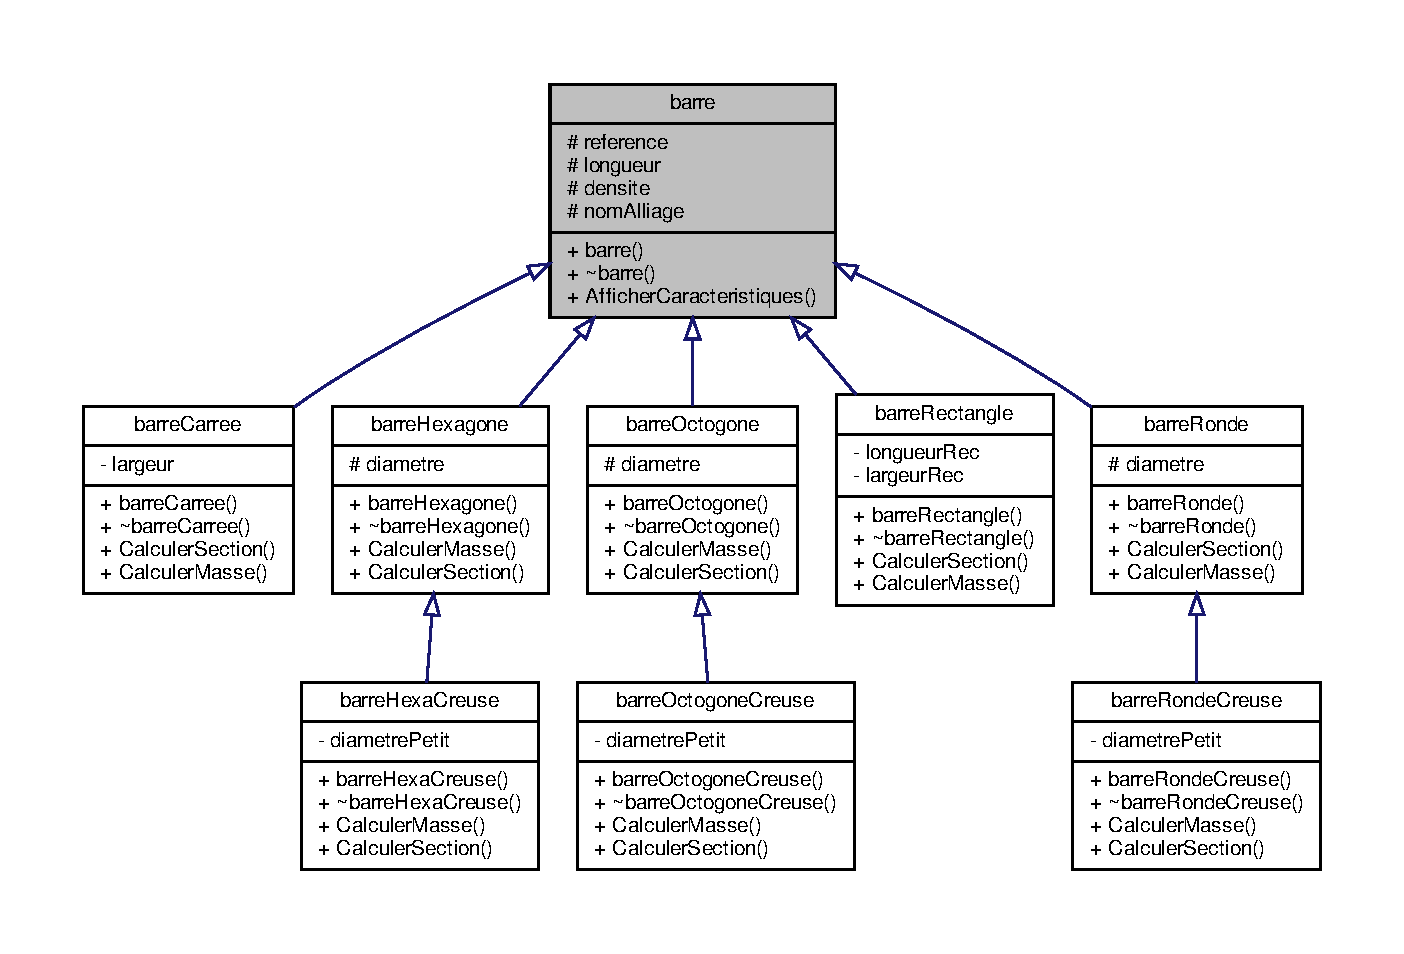
\includegraphics[width=350pt]{classbarre__inherit__graph}
\end{center}
\end{figure}


Graphe de collaboration de barre\+:
\nopagebreak
\begin{figure}[H]
\begin{center}
\leavevmode
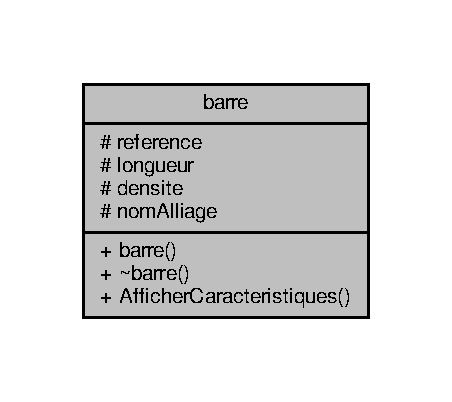
\includegraphics[width=217pt]{classbarre__coll__graph}
\end{center}
\end{figure}
\subsection*{Fonctions membres publiques}
\begin{DoxyCompactItemize}
\item 
\hyperlink{classbarre_a110cf86db5f686f1fc2dc3472c1d27a5}{barre} (const string \+\_\+reference, const int \+\_\+longueur, const float \+\_\+densite, const string \hyperlink{classbarre_ace8c42f734a0b6046dc7c6ef0e1226f5}{nom\+Alliage})
\begin{DoxyCompactList}\small\item\em \hyperlink{classbarre_a110cf86db5f686f1fc2dc3472c1d27a5}{barre\+::barre} \end{DoxyCompactList}\item 
\hyperlink{classbarre_aad01e01332f1c25ed92b9ea5626a1c33}{$\sim$barre} ()
\begin{DoxyCompactList}\small\item\em \hyperlink{classbarre_aad01e01332f1c25ed92b9ea5626a1c33}{barre\+::$\sim$barre} \end{DoxyCompactList}\item 
void \hyperlink{classbarre_a65fd04c5ba981c50569d582a1b5f35b0}{Afficher\+Caracteristiques} ()
\begin{DoxyCompactList}\small\item\em \hyperlink{classbarre_a65fd04c5ba981c50569d582a1b5f35b0}{barre\+::\+Afficher\+Caracteristiques} \end{DoxyCompactList}\end{DoxyCompactItemize}
\subsection*{Attributs protégés}
\begin{DoxyCompactItemize}
\item 
string \hyperlink{classbarre_a078de0af40f717a1ab145687bda7928d}{reference}
\item 
float \hyperlink{classbarre_acb72acedfbb8c691f29baae6389b8306}{longueur}
\item 
float \hyperlink{classbarre_a41bef49c05b7c407272055ce116f5d9d}{densite}
\item 
string \hyperlink{classbarre_ace8c42f734a0b6046dc7c6ef0e1226f5}{nom\+Alliage}
\end{DoxyCompactItemize}


\subsection{Description détaillée}
The barre class. 

\subsection{Documentation des constructeurs et destructeur}
\mbox{\Hypertarget{classbarre_a110cf86db5f686f1fc2dc3472c1d27a5}\label{classbarre_a110cf86db5f686f1fc2dc3472c1d27a5}} 
\index{barre@{barre}!barre@{barre}}
\index{barre@{barre}!barre@{barre}}
\subsubsection{\texorpdfstring{barre()}{barre()}}
{\footnotesize\ttfamily barre\+::barre (\begin{DoxyParamCaption}\item[{const string}]{\+\_\+reference,  }\item[{const int}]{\+\_\+longueur,  }\item[{const float}]{\+\_\+densite,  }\item[{const string}]{\+\_\+nom\+Alliage }\end{DoxyParamCaption})}



\hyperlink{classbarre_a110cf86db5f686f1fc2dc3472c1d27a5}{barre\+::barre} 


\begin{DoxyParams}{Paramètres}
{\em \+\_\+reference} & \\
\hline
{\em \+\_\+longueur} & \\
\hline
{\em \+\_\+densite} & \\
\hline
{\em \+\_\+nom\+Alliage} & \\
\hline
\end{DoxyParams}
Constructeur de la classe barre \mbox{\Hypertarget{classbarre_aad01e01332f1c25ed92b9ea5626a1c33}\label{classbarre_aad01e01332f1c25ed92b9ea5626a1c33}} 
\index{barre@{barre}!````~barre@{$\sim$barre}}
\index{````~barre@{$\sim$barre}!barre@{barre}}
\subsubsection{\texorpdfstring{$\sim$barre()}{~barre()}}
{\footnotesize\ttfamily barre\+::$\sim$barre (\begin{DoxyParamCaption}{ }\end{DoxyParamCaption})}



\hyperlink{classbarre_aad01e01332f1c25ed92b9ea5626a1c33}{barre\+::$\sim$barre} 

destructeur classe barre 

\subsection{Documentation des fonctions membres}
\mbox{\Hypertarget{classbarre_a65fd04c5ba981c50569d582a1b5f35b0}\label{classbarre_a65fd04c5ba981c50569d582a1b5f35b0}} 
\index{barre@{barre}!Afficher\+Caracteristiques@{Afficher\+Caracteristiques}}
\index{Afficher\+Caracteristiques@{Afficher\+Caracteristiques}!barre@{barre}}
\subsubsection{\texorpdfstring{Afficher\+Caracteristiques()}{AfficherCaracteristiques()}}
{\footnotesize\ttfamily void barre\+::\+Afficher\+Caracteristiques (\begin{DoxyParamCaption}{ }\end{DoxyParamCaption})}



\hyperlink{classbarre_a65fd04c5ba981c50569d582a1b5f35b0}{barre\+::\+Afficher\+Caracteristiques} 

methode afficher les caracteristique 

\subsection{Documentation des données membres}
\mbox{\Hypertarget{classbarre_a41bef49c05b7c407272055ce116f5d9d}\label{classbarre_a41bef49c05b7c407272055ce116f5d9d}} 
\index{barre@{barre}!densite@{densite}}
\index{densite@{densite}!barre@{barre}}
\subsubsection{\texorpdfstring{densite}{densite}}
{\footnotesize\ttfamily float barre\+::densite\hspace{0.3cm}{\ttfamily [protected]}}

\mbox{\Hypertarget{classbarre_acb72acedfbb8c691f29baae6389b8306}\label{classbarre_acb72acedfbb8c691f29baae6389b8306}} 
\index{barre@{barre}!longueur@{longueur}}
\index{longueur@{longueur}!barre@{barre}}
\subsubsection{\texorpdfstring{longueur}{longueur}}
{\footnotesize\ttfamily float barre\+::longueur\hspace{0.3cm}{\ttfamily [protected]}}

\mbox{\Hypertarget{classbarre_ace8c42f734a0b6046dc7c6ef0e1226f5}\label{classbarre_ace8c42f734a0b6046dc7c6ef0e1226f5}} 
\index{barre@{barre}!nom\+Alliage@{nom\+Alliage}}
\index{nom\+Alliage@{nom\+Alliage}!barre@{barre}}
\subsubsection{\texorpdfstring{nom\+Alliage}{nomAlliage}}
{\footnotesize\ttfamily string barre\+::nom\+Alliage\hspace{0.3cm}{\ttfamily [protected]}}

\mbox{\Hypertarget{classbarre_a078de0af40f717a1ab145687bda7928d}\label{classbarre_a078de0af40f717a1ab145687bda7928d}} 
\index{barre@{barre}!reference@{reference}}
\index{reference@{reference}!barre@{barre}}
\subsubsection{\texorpdfstring{reference}{reference}}
{\footnotesize\ttfamily string barre\+::reference\hspace{0.3cm}{\ttfamily [protected]}}



La documentation de cette classe a été générée à partir des fichiers suivants \+:\begin{DoxyCompactItemize}
\item 
T\+D\+\_\+\+Barre/\hyperlink{barre_8h}{barre.\+h}\item 
T\+D\+\_\+\+Barre/\hyperlink{barre_8cpp}{barre.\+cpp}\end{DoxyCompactItemize}

\hypertarget{classbarre_carree}{}\section{Référence de la classe barre\+Carree}
\label{classbarre_carree}\index{barre\+Carree@{barre\+Carree}}


The \hyperlink{classbarre_carree}{barre\+Carree} class.  




{\ttfamily \#include $<$barrecaree.\+h$>$}



Graphe d\textquotesingle{}héritage de barre\+Carree\+:
\nopagebreak
\begin{figure}[H]
\begin{center}
\leavevmode
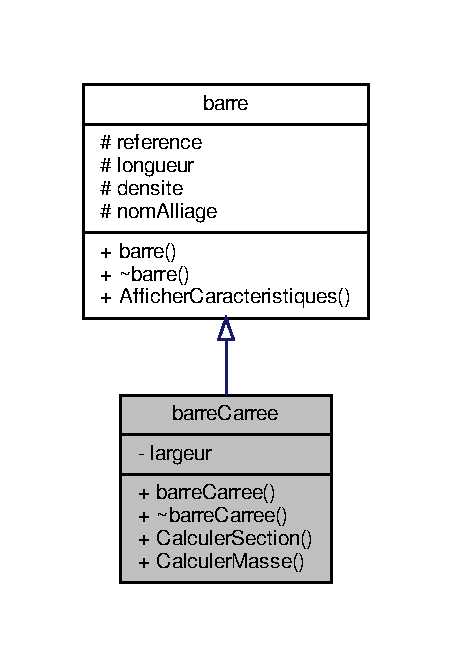
\includegraphics[width=217pt]{classbarre_carree__inherit__graph}
\end{center}
\end{figure}


Graphe de collaboration de barre\+Carree\+:
\nopagebreak
\begin{figure}[H]
\begin{center}
\leavevmode
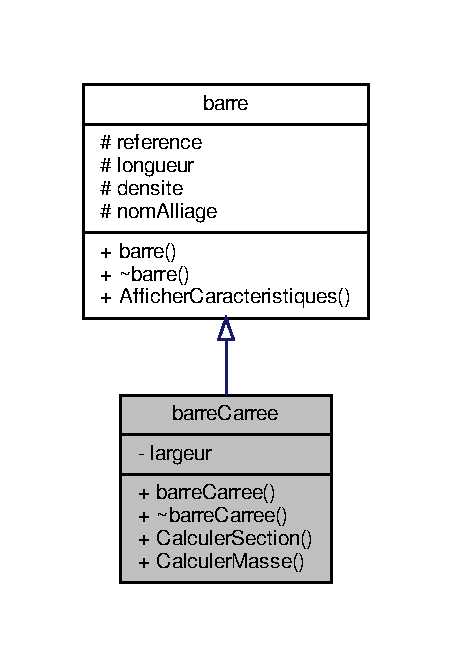
\includegraphics[width=217pt]{classbarre_carree__coll__graph}
\end{center}
\end{figure}
\subsection*{Fonctions membres publiques}
\begin{DoxyCompactItemize}
\item 
\hyperlink{classbarre_carree_aff83dbd539a72ea608e0d976fe021e5a}{barre\+Carree} (const string \+\_\+reference, const int \+\_\+longueur, const float \+\_\+densite, const string \+\_\+nom\+Alliage, const int \+\_\+largeur)
\begin{DoxyCompactList}\small\item\em \hyperlink{classbarre_carree_aff83dbd539a72ea608e0d976fe021e5a}{barre\+Carree\+::barre\+Carree} \end{DoxyCompactList}\item 
\hyperlink{classbarre_carree_a586fa64f84b0d977472f520222ae7554}{$\sim$barre\+Carree} ()
\begin{DoxyCompactList}\small\item\em \hyperlink{classbarre_carree_a586fa64f84b0d977472f520222ae7554}{barre\+Carree\+::$\sim$barre\+Carree} \end{DoxyCompactList}\item 
double \hyperlink{classbarre_carree_ab7965489abcbac7f9e7d108f801c95e0}{Calculer\+Section} ()
\begin{DoxyCompactList}\small\item\em \hyperlink{classbarre_carree_ab7965489abcbac7f9e7d108f801c95e0}{barre\+Carree\+::\+Calculer\+Section} \end{DoxyCompactList}\item 
double \hyperlink{classbarre_carree_abc27ea4b81f19f699656dd0c037938ae}{Calculer\+Masse} ()
\begin{DoxyCompactList}\small\item\em \hyperlink{classbarre_carree_abc27ea4b81f19f699656dd0c037938ae}{barre\+Carree\+::\+Calculer\+Masse} \end{DoxyCompactList}\end{DoxyCompactItemize}
\subsection*{Attributs privés}
\begin{DoxyCompactItemize}
\item 
int \hyperlink{classbarre_carree_ad2090886607c393f6222239f3efaff0d}{largeur}
\end{DoxyCompactItemize}
\subsection*{Membres hérités additionnels}


\subsection{Description détaillée}
The \hyperlink{classbarre_carree}{barre\+Carree} class. 

\subsection{Documentation des constructeurs et destructeur}
\mbox{\Hypertarget{classbarre_carree_aff83dbd539a72ea608e0d976fe021e5a}\label{classbarre_carree_aff83dbd539a72ea608e0d976fe021e5a}} 
\index{barre\+Carree@{barre\+Carree}!barre\+Carree@{barre\+Carree}}
\index{barre\+Carree@{barre\+Carree}!barre\+Carree@{barre\+Carree}}
\subsubsection{\texorpdfstring{barre\+Carree()}{barreCarree()}}
{\footnotesize\ttfamily barre\+Carree\+::barre\+Carree (\begin{DoxyParamCaption}\item[{const string}]{\+\_\+reference,  }\item[{const int}]{\+\_\+longueur,  }\item[{const float}]{\+\_\+densite,  }\item[{const string}]{\+\_\+nom\+Alliage,  }\item[{const int}]{\+\_\+largeur }\end{DoxyParamCaption})}



\hyperlink{classbarre_carree_aff83dbd539a72ea608e0d976fe021e5a}{barre\+Carree\+::barre\+Carree} 


\begin{DoxyParams}{Paramètres}
{\em \+\_\+reference} & \\
\hline
{\em \+\_\+longueur} & \\
\hline
{\em \+\_\+densite} & \\
\hline
{\em \+\_\+nom\+Alliage} & \\
\hline
{\em \+\_\+largeur} & \\
\hline
\end{DoxyParams}
Constructeur classe Barre\+Carree \mbox{\Hypertarget{classbarre_carree_a586fa64f84b0d977472f520222ae7554}\label{classbarre_carree_a586fa64f84b0d977472f520222ae7554}} 
\index{barre\+Carree@{barre\+Carree}!````~barre\+Carree@{$\sim$barre\+Carree}}
\index{````~barre\+Carree@{$\sim$barre\+Carree}!barre\+Carree@{barre\+Carree}}
\subsubsection{\texorpdfstring{$\sim$barre\+Carree()}{~barreCarree()}}
{\footnotesize\ttfamily barre\+Carree\+::$\sim$barre\+Carree (\begin{DoxyParamCaption}{ }\end{DoxyParamCaption})}



\hyperlink{classbarre_carree_a586fa64f84b0d977472f520222ae7554}{barre\+Carree\+::$\sim$barre\+Carree} 

Destructeur Classe Barre\+Carree 

\subsection{Documentation des fonctions membres}
\mbox{\Hypertarget{classbarre_carree_abc27ea4b81f19f699656dd0c037938ae}\label{classbarre_carree_abc27ea4b81f19f699656dd0c037938ae}} 
\index{barre\+Carree@{barre\+Carree}!Calculer\+Masse@{Calculer\+Masse}}
\index{Calculer\+Masse@{Calculer\+Masse}!barre\+Carree@{barre\+Carree}}
\subsubsection{\texorpdfstring{Calculer\+Masse()}{CalculerMasse()}}
{\footnotesize\ttfamily double barre\+Carree\+::\+Calculer\+Masse (\begin{DoxyParamCaption}{ }\end{DoxyParamCaption})}



\hyperlink{classbarre_carree_abc27ea4b81f19f699656dd0c037938ae}{barre\+Carree\+::\+Calculer\+Masse} 

\begin{DoxyReturn}{Renvoie}

\end{DoxyReturn}
Methode Calculer\+Masse \mbox{\Hypertarget{classbarre_carree_ab7965489abcbac7f9e7d108f801c95e0}\label{classbarre_carree_ab7965489abcbac7f9e7d108f801c95e0}} 
\index{barre\+Carree@{barre\+Carree}!Calculer\+Section@{Calculer\+Section}}
\index{Calculer\+Section@{Calculer\+Section}!barre\+Carree@{barre\+Carree}}
\subsubsection{\texorpdfstring{Calculer\+Section()}{CalculerSection()}}
{\footnotesize\ttfamily double barre\+Carree\+::\+Calculer\+Section (\begin{DoxyParamCaption}{ }\end{DoxyParamCaption})}



\hyperlink{classbarre_carree_ab7965489abcbac7f9e7d108f801c95e0}{barre\+Carree\+::\+Calculer\+Section} 

\begin{DoxyReturn}{Renvoie}

\end{DoxyReturn}
Methode Calculer\+Section 

\subsection{Documentation des données membres}
\mbox{\Hypertarget{classbarre_carree_ad2090886607c393f6222239f3efaff0d}\label{classbarre_carree_ad2090886607c393f6222239f3efaff0d}} 
\index{barre\+Carree@{barre\+Carree}!largeur@{largeur}}
\index{largeur@{largeur}!barre\+Carree@{barre\+Carree}}
\subsubsection{\texorpdfstring{largeur}{largeur}}
{\footnotesize\ttfamily int barre\+Carree\+::largeur\hspace{0.3cm}{\ttfamily [private]}}



La documentation de cette classe a été générée à partir des fichiers suivants \+:\begin{DoxyCompactItemize}
\item 
T\+D\+\_\+\+Barre/\hyperlink{barrecaree_8h}{barrecaree.\+h}\item 
T\+D\+\_\+\+Barre/\hyperlink{barrecaree_8cpp}{barrecaree.\+cpp}\end{DoxyCompactItemize}

\hypertarget{classbarre_hexa_creuse}{}\section{Référence de la classe barre\+Hexa\+Creuse}
\label{classbarre_hexa_creuse}\index{barre\+Hexa\+Creuse@{barre\+Hexa\+Creuse}}


The \hyperlink{classbarre_hexa_creuse}{barre\+Hexa\+Creuse} class.  




{\ttfamily \#include $<$barrehexacreuse.\+h$>$}



Graphe d\textquotesingle{}héritage de barre\+Hexa\+Creuse\+:
\nopagebreak
\begin{figure}[H]
\begin{center}
\leavevmode
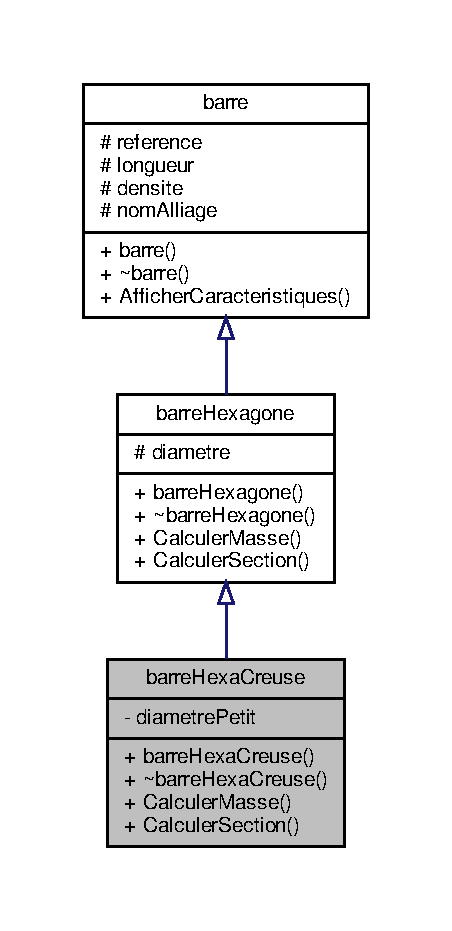
\includegraphics[width=217pt]{classbarre_hexa_creuse__inherit__graph}
\end{center}
\end{figure}


Graphe de collaboration de barre\+Hexa\+Creuse\+:
\nopagebreak
\begin{figure}[H]
\begin{center}
\leavevmode
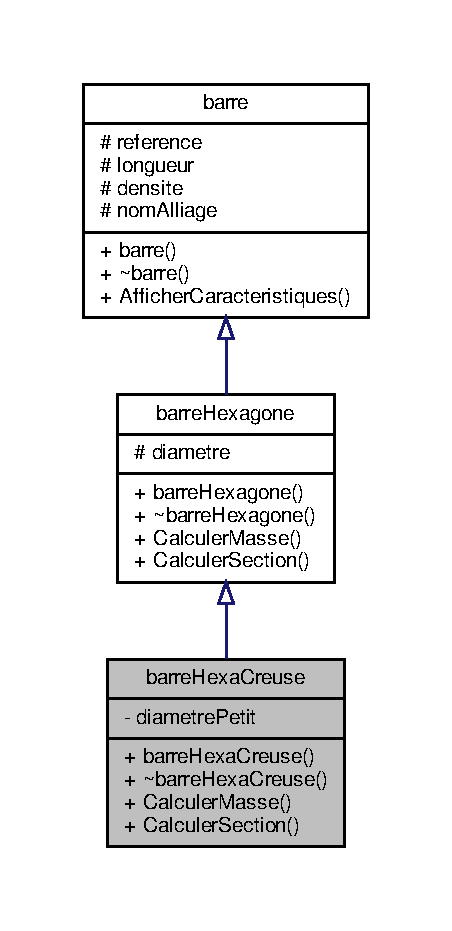
\includegraphics[width=217pt]{classbarre_hexa_creuse__coll__graph}
\end{center}
\end{figure}
\subsection*{Fonctions membres publiques}
\begin{DoxyCompactItemize}
\item 
\hyperlink{classbarre_hexa_creuse_a0da420fa29dd2b947661958729f1f0d7}{barre\+Hexa\+Creuse} (const string \+\_\+reference, const int \+\_\+longueur, const float \+\_\+densite, const string \+\_\+nom\+Alliage, const double \+\_\+diametre, const double \+\_\+diametre\+Petit)
\begin{DoxyCompactList}\small\item\em \hyperlink{classbarre_hexa_creuse_a0da420fa29dd2b947661958729f1f0d7}{barre\+Hexa\+Creuse\+::barre\+Hexa\+Creuse} \end{DoxyCompactList}\item 
\hyperlink{classbarre_hexa_creuse_a5b51540579b5268f23dbcf8e5db04458}{$\sim$barre\+Hexa\+Creuse} ()
\begin{DoxyCompactList}\small\item\em \hyperlink{classbarre_hexa_creuse_a5b51540579b5268f23dbcf8e5db04458}{barre\+Hexa\+Creuse\+::$\sim$barre\+Hexa\+Creuse} \end{DoxyCompactList}\item 
double \hyperlink{classbarre_hexa_creuse_a0d524ad6862407dc9128c7163b22a0ca}{Calculer\+Masse} ()
\begin{DoxyCompactList}\small\item\em \hyperlink{classbarre_hexa_creuse_a0d524ad6862407dc9128c7163b22a0ca}{barre\+Hexa\+Creuse\+::\+Calculer\+Masse} \end{DoxyCompactList}\item 
double \hyperlink{classbarre_hexa_creuse_a205ab8a47da16cd0eb63770bcd911b90}{Calculer\+Section} ()
\begin{DoxyCompactList}\small\item\em \hyperlink{classbarre_hexa_creuse_a205ab8a47da16cd0eb63770bcd911b90}{barre\+Hexa\+Creuse\+::\+Calculer\+Section} \end{DoxyCompactList}\end{DoxyCompactItemize}
\subsection*{Attributs privés}
\begin{DoxyCompactItemize}
\item 
double \hyperlink{classbarre_hexa_creuse_a9d3319db26ff56f7b27c374535a89a6d}{diametre\+Petit}
\end{DoxyCompactItemize}
\subsection*{Membres hérités additionnels}


\subsection{Description détaillée}
The \hyperlink{classbarre_hexa_creuse}{barre\+Hexa\+Creuse} class. 

Definition de la classebarre\+Hexa\+Creuse 

\subsection{Documentation des constructeurs et destructeur}
\mbox{\Hypertarget{classbarre_hexa_creuse_a0da420fa29dd2b947661958729f1f0d7}\label{classbarre_hexa_creuse_a0da420fa29dd2b947661958729f1f0d7}} 
\index{barre\+Hexa\+Creuse@{barre\+Hexa\+Creuse}!barre\+Hexa\+Creuse@{barre\+Hexa\+Creuse}}
\index{barre\+Hexa\+Creuse@{barre\+Hexa\+Creuse}!barre\+Hexa\+Creuse@{barre\+Hexa\+Creuse}}
\subsubsection{\texorpdfstring{barre\+Hexa\+Creuse()}{barreHexaCreuse()}}
{\footnotesize\ttfamily barre\+Hexa\+Creuse\+::barre\+Hexa\+Creuse (\begin{DoxyParamCaption}\item[{const string}]{\+\_\+reference,  }\item[{const int}]{\+\_\+longueur,  }\item[{const float}]{\+\_\+densite,  }\item[{const string}]{\+\_\+nom\+Alliage,  }\item[{const double}]{\+\_\+diametre,  }\item[{const double}]{\+\_\+diametre\+Petit }\end{DoxyParamCaption})}



\hyperlink{classbarre_hexa_creuse_a0da420fa29dd2b947661958729f1f0d7}{barre\+Hexa\+Creuse\+::barre\+Hexa\+Creuse} 


\begin{DoxyParams}{Paramètres}
{\em \+\_\+reference} & \\
\hline
{\em \+\_\+longueur} & \\
\hline
{\em \+\_\+densite} & \\
\hline
{\em \+\_\+nom\+Alliage} & \\
\hline
{\em \+\_\+diametre} & \\
\hline
{\em \+\_\+diametre\+Petit} & \\
\hline
\end{DoxyParams}
\mbox{\Hypertarget{classbarre_hexa_creuse_a5b51540579b5268f23dbcf8e5db04458}\label{classbarre_hexa_creuse_a5b51540579b5268f23dbcf8e5db04458}} 
\index{barre\+Hexa\+Creuse@{barre\+Hexa\+Creuse}!````~barre\+Hexa\+Creuse@{$\sim$barre\+Hexa\+Creuse}}
\index{````~barre\+Hexa\+Creuse@{$\sim$barre\+Hexa\+Creuse}!barre\+Hexa\+Creuse@{barre\+Hexa\+Creuse}}
\subsubsection{\texorpdfstring{$\sim$barre\+Hexa\+Creuse()}{~barreHexaCreuse()}}
{\footnotesize\ttfamily barre\+Hexa\+Creuse\+::$\sim$barre\+Hexa\+Creuse (\begin{DoxyParamCaption}{ }\end{DoxyParamCaption})}



\hyperlink{classbarre_hexa_creuse_a5b51540579b5268f23dbcf8e5db04458}{barre\+Hexa\+Creuse\+::$\sim$barre\+Hexa\+Creuse} 

Destructeur de la classe \hyperlink{classbarre_hexa_creuse}{barre\+Hexa\+Creuse} 

\subsection{Documentation des fonctions membres}
\mbox{\Hypertarget{classbarre_hexa_creuse_a0d524ad6862407dc9128c7163b22a0ca}\label{classbarre_hexa_creuse_a0d524ad6862407dc9128c7163b22a0ca}} 
\index{barre\+Hexa\+Creuse@{barre\+Hexa\+Creuse}!Calculer\+Masse@{Calculer\+Masse}}
\index{Calculer\+Masse@{Calculer\+Masse}!barre\+Hexa\+Creuse@{barre\+Hexa\+Creuse}}
\subsubsection{\texorpdfstring{Calculer\+Masse()}{CalculerMasse()}}
{\footnotesize\ttfamily double barre\+Hexa\+Creuse\+::\+Calculer\+Masse (\begin{DoxyParamCaption}{ }\end{DoxyParamCaption})}



\hyperlink{classbarre_hexa_creuse_a0d524ad6862407dc9128c7163b22a0ca}{barre\+Hexa\+Creuse\+::\+Calculer\+Masse} 

\begin{DoxyReturn}{Renvoie}

\end{DoxyReturn}
Methode Calculer\+Masse qui renvoie la masse \mbox{\Hypertarget{classbarre_hexa_creuse_a205ab8a47da16cd0eb63770bcd911b90}\label{classbarre_hexa_creuse_a205ab8a47da16cd0eb63770bcd911b90}} 
\index{barre\+Hexa\+Creuse@{barre\+Hexa\+Creuse}!Calculer\+Section@{Calculer\+Section}}
\index{Calculer\+Section@{Calculer\+Section}!barre\+Hexa\+Creuse@{barre\+Hexa\+Creuse}}
\subsubsection{\texorpdfstring{Calculer\+Section()}{CalculerSection()}}
{\footnotesize\ttfamily double barre\+Hexa\+Creuse\+::\+Calculer\+Section (\begin{DoxyParamCaption}{ }\end{DoxyParamCaption})}



\hyperlink{classbarre_hexa_creuse_a205ab8a47da16cd0eb63770bcd911b90}{barre\+Hexa\+Creuse\+::\+Calculer\+Section} 

\begin{DoxyReturn}{Renvoie}

\end{DoxyReturn}
Methode Calculer\+Section qui renvoie la valeur de la section 

\subsection{Documentation des données membres}
\mbox{\Hypertarget{classbarre_hexa_creuse_a9d3319db26ff56f7b27c374535a89a6d}\label{classbarre_hexa_creuse_a9d3319db26ff56f7b27c374535a89a6d}} 
\index{barre\+Hexa\+Creuse@{barre\+Hexa\+Creuse}!diametre\+Petit@{diametre\+Petit}}
\index{diametre\+Petit@{diametre\+Petit}!barre\+Hexa\+Creuse@{barre\+Hexa\+Creuse}}
\subsubsection{\texorpdfstring{diametre\+Petit}{diametrePetit}}
{\footnotesize\ttfamily double barre\+Hexa\+Creuse\+::diametre\+Petit\hspace{0.3cm}{\ttfamily [private]}}



La documentation de cette classe a été générée à partir des fichiers suivants \+:\begin{DoxyCompactItemize}
\item 
T\+D\+\_\+\+Barre/\hyperlink{barrehexacreuse_8h}{barrehexacreuse.\+h}\item 
T\+D\+\_\+\+Barre/\hyperlink{barrehexacreuse_8cpp}{barrehexacreuse.\+cpp}\end{DoxyCompactItemize}

\hypertarget{classbarre_hexagone}{}\section{Référence de la classe barre\+Hexagone}
\label{classbarre_hexagone}\index{barre\+Hexagone@{barre\+Hexagone}}


The \hyperlink{classbarre_hexagone}{barre\+Hexagone} class.  




{\ttfamily \#include $<$barrehexagone.\+h$>$}



Graphe d\textquotesingle{}héritage de barre\+Hexagone\+:
\nopagebreak
\begin{figure}[H]
\begin{center}
\leavevmode
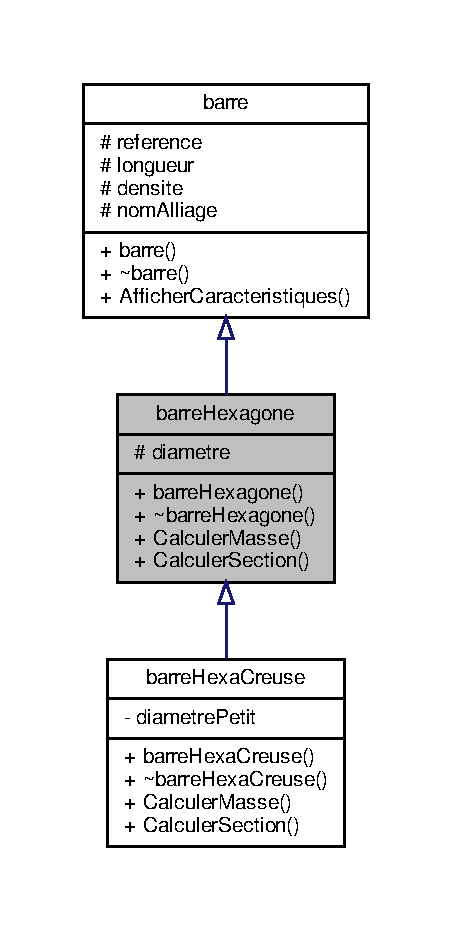
\includegraphics[width=217pt]{classbarre_hexagone__inherit__graph}
\end{center}
\end{figure}


Graphe de collaboration de barre\+Hexagone\+:
\nopagebreak
\begin{figure}[H]
\begin{center}
\leavevmode
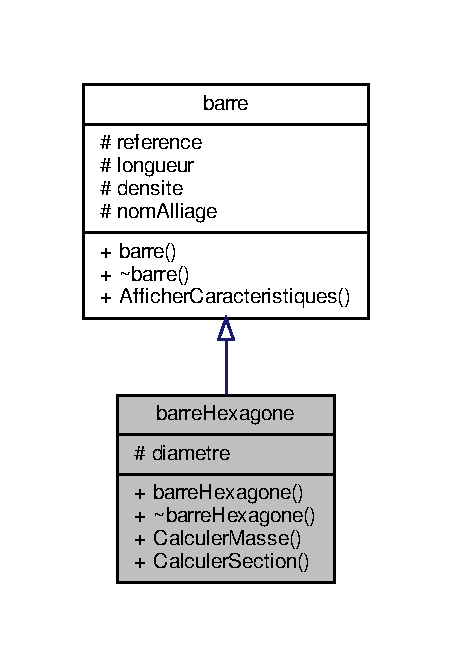
\includegraphics[width=217pt]{classbarre_hexagone__coll__graph}
\end{center}
\end{figure}
\subsection*{Fonctions membres publiques}
\begin{DoxyCompactItemize}
\item 
\hyperlink{classbarre_hexagone_ae4c0f6eeac2af444aa99d6331916046d}{barre\+Hexagone} (const string \+\_\+reference, const int \+\_\+longueur, const float \+\_\+densite, const string \+\_\+nom\+Alliage, const double \+\_\+diametre)
\begin{DoxyCompactList}\small\item\em \hyperlink{classbarre_hexagone_ae4c0f6eeac2af444aa99d6331916046d}{barre\+Hexagone\+::barre\+Hexagone} \end{DoxyCompactList}\item 
\hyperlink{classbarre_hexagone_a525e2b1acce9f429ab4aad471b7e86da}{$\sim$barre\+Hexagone} ()
\begin{DoxyCompactList}\small\item\em \hyperlink{classbarre_hexagone_a525e2b1acce9f429ab4aad471b7e86da}{barre\+Hexagone\+::$\sim$barre\+Hexagone} \end{DoxyCompactList}\item 
double \hyperlink{classbarre_hexagone_a310610a3d03be6010899d1741a853b5b}{Calculer\+Masse} ()
\item 
double \hyperlink{classbarre_hexagone_a456a7b2330ae62eac9be943d6cfadeca}{Calculer\+Section} ()
\begin{DoxyCompactList}\small\item\em \hyperlink{classbarre_hexagone_a456a7b2330ae62eac9be943d6cfadeca}{barre\+Hexagone\+::\+Calculer\+Section} \end{DoxyCompactList}\end{DoxyCompactItemize}
\subsection*{Attributs protégés}
\begin{DoxyCompactItemize}
\item 
double \hyperlink{classbarre_hexagone_ac91cbf9757ea749c85603df250abb62c}{diametre}
\end{DoxyCompactItemize}


\subsection{Description détaillée}
The \hyperlink{classbarre_hexagone}{barre\+Hexagone} class. 

Definition de la classe Barre\+Hexagone qui herite de barre 

\subsection{Documentation des constructeurs et destructeur}
\mbox{\Hypertarget{classbarre_hexagone_ae4c0f6eeac2af444aa99d6331916046d}\label{classbarre_hexagone_ae4c0f6eeac2af444aa99d6331916046d}} 
\index{barre\+Hexagone@{barre\+Hexagone}!barre\+Hexagone@{barre\+Hexagone}}
\index{barre\+Hexagone@{barre\+Hexagone}!barre\+Hexagone@{barre\+Hexagone}}
\subsubsection{\texorpdfstring{barre\+Hexagone()}{barreHexagone()}}
{\footnotesize\ttfamily barre\+Hexagone\+::barre\+Hexagone (\begin{DoxyParamCaption}\item[{const string}]{\+\_\+reference,  }\item[{const int}]{\+\_\+longueur,  }\item[{const float}]{\+\_\+densite,  }\item[{const string}]{\+\_\+nom\+Alliage,  }\item[{const double}]{\+\_\+diametre }\end{DoxyParamCaption})}



\hyperlink{classbarre_hexagone_ae4c0f6eeac2af444aa99d6331916046d}{barre\+Hexagone\+::barre\+Hexagone} 


\begin{DoxyParams}{Paramètres}
{\em \+\_\+reference} & \\
\hline
{\em \+\_\+longueur} & \\
\hline
{\em \+\_\+densite} & \\
\hline
{\em \+\_\+nom\+Alliage} & \\
\hline
{\em \+\_\+diametre} & \\
\hline
\end{DoxyParams}
Constructeur de la classe Barre Hexagone \mbox{\Hypertarget{classbarre_hexagone_a525e2b1acce9f429ab4aad471b7e86da}\label{classbarre_hexagone_a525e2b1acce9f429ab4aad471b7e86da}} 
\index{barre\+Hexagone@{barre\+Hexagone}!````~barre\+Hexagone@{$\sim$barre\+Hexagone}}
\index{````~barre\+Hexagone@{$\sim$barre\+Hexagone}!barre\+Hexagone@{barre\+Hexagone}}
\subsubsection{\texorpdfstring{$\sim$barre\+Hexagone()}{~barreHexagone()}}
{\footnotesize\ttfamily barre\+Hexagone\+::$\sim$barre\+Hexagone (\begin{DoxyParamCaption}{ }\end{DoxyParamCaption})}



\hyperlink{classbarre_hexagone_a525e2b1acce9f429ab4aad471b7e86da}{barre\+Hexagone\+::$\sim$barre\+Hexagone} 

Destructeur de la classe Barre Hexagone 

\subsection{Documentation des fonctions membres}
\mbox{\Hypertarget{classbarre_hexagone_a310610a3d03be6010899d1741a853b5b}\label{classbarre_hexagone_a310610a3d03be6010899d1741a853b5b}} 
\index{barre\+Hexagone@{barre\+Hexagone}!Calculer\+Masse@{Calculer\+Masse}}
\index{Calculer\+Masse@{Calculer\+Masse}!barre\+Hexagone@{barre\+Hexagone}}
\subsubsection{\texorpdfstring{Calculer\+Masse()}{CalculerMasse()}}
{\footnotesize\ttfamily double barre\+Hexagone\+::\+Calculer\+Masse (\begin{DoxyParamCaption}{ }\end{DoxyParamCaption})}

On change le type de longueur et densite en double \mbox{\Hypertarget{classbarre_hexagone_a456a7b2330ae62eac9be943d6cfadeca}\label{classbarre_hexagone_a456a7b2330ae62eac9be943d6cfadeca}} 
\index{barre\+Hexagone@{barre\+Hexagone}!Calculer\+Section@{Calculer\+Section}}
\index{Calculer\+Section@{Calculer\+Section}!barre\+Hexagone@{barre\+Hexagone}}
\subsubsection{\texorpdfstring{Calculer\+Section()}{CalculerSection()}}
{\footnotesize\ttfamily double barre\+Hexagone\+::\+Calculer\+Section (\begin{DoxyParamCaption}{ }\end{DoxyParamCaption})}



\hyperlink{classbarre_hexagone_a456a7b2330ae62eac9be943d6cfadeca}{barre\+Hexagone\+::\+Calculer\+Section} 

\begin{DoxyReturn}{Renvoie}

\end{DoxyReturn}
Methode Calculer\+Section qui renvoie la Section 

\subsection{Documentation des données membres}
\mbox{\Hypertarget{classbarre_hexagone_ac91cbf9757ea749c85603df250abb62c}\label{classbarre_hexagone_ac91cbf9757ea749c85603df250abb62c}} 
\index{barre\+Hexagone@{barre\+Hexagone}!diametre@{diametre}}
\index{diametre@{diametre}!barre\+Hexagone@{barre\+Hexagone}}
\subsubsection{\texorpdfstring{diametre}{diametre}}
{\footnotesize\ttfamily double barre\+Hexagone\+::diametre\hspace{0.3cm}{\ttfamily [protected]}}



La documentation de cette classe a été générée à partir des fichiers suivants \+:\begin{DoxyCompactItemize}
\item 
T\+D\+\_\+\+Barre/\hyperlink{barrehexagone_8h}{barrehexagone.\+h}\item 
T\+D\+\_\+\+Barre/\hyperlink{barrehexagone_8cpp}{barrehexagone.\+cpp}\end{DoxyCompactItemize}

\hypertarget{classbarre_octogone}{}\section{Référence de la classe barre\+Octogone}
\label{classbarre_octogone}\index{barre\+Octogone@{barre\+Octogone}}


The \hyperlink{classbarre_octogone}{barre\+Octogone} class.  




{\ttfamily \#include $<$barreoctogone.\+h$>$}



Graphe d\textquotesingle{}héritage de barre\+Octogone\+:
\nopagebreak
\begin{figure}[H]
\begin{center}
\leavevmode
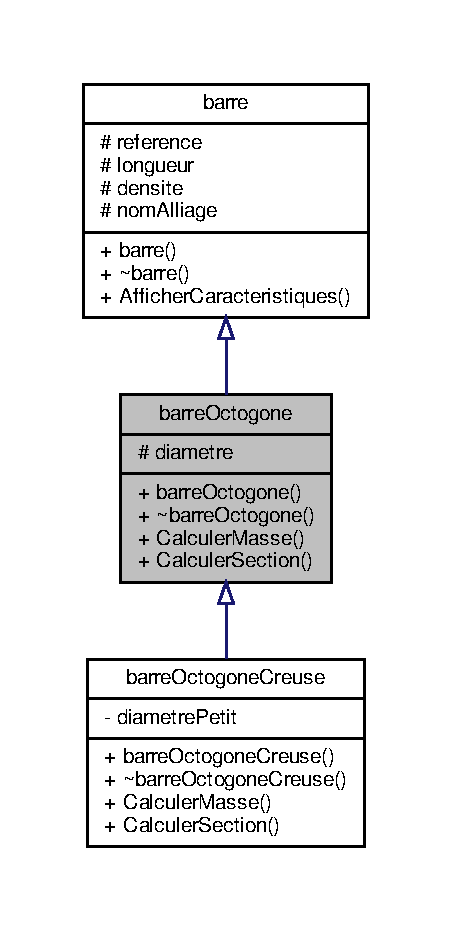
\includegraphics[width=217pt]{classbarre_octogone__inherit__graph}
\end{center}
\end{figure}


Graphe de collaboration de barre\+Octogone\+:
\nopagebreak
\begin{figure}[H]
\begin{center}
\leavevmode
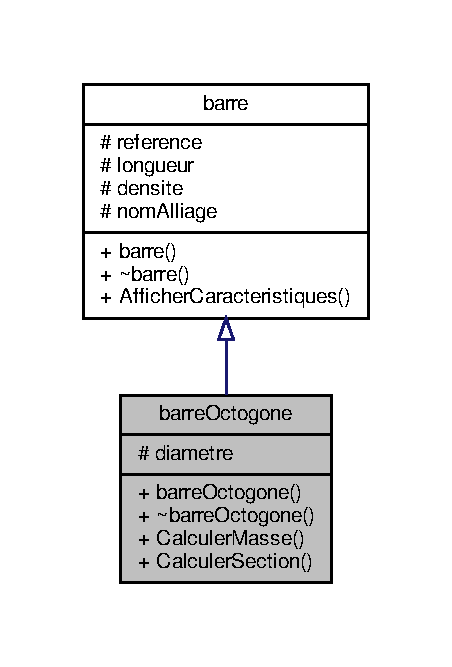
\includegraphics[width=217pt]{classbarre_octogone__coll__graph}
\end{center}
\end{figure}
\subsection*{Fonctions membres publiques}
\begin{DoxyCompactItemize}
\item 
\hyperlink{classbarre_octogone_a155858ba0e9b2b00a99c96391cb95626}{barre\+Octogone} (const string \+\_\+reference, const int \+\_\+longueur, const float \+\_\+densite, const string \+\_\+nom\+Alliage, const double \+\_\+diametre)
\begin{DoxyCompactList}\small\item\em \hyperlink{classbarre_octogone_a155858ba0e9b2b00a99c96391cb95626}{barre\+Octogone\+::barre\+Octogone} \end{DoxyCompactList}\item 
\hyperlink{classbarre_octogone_ace0c5f7ff3f012b530679e0784a5a577}{$\sim$barre\+Octogone} ()
\begin{DoxyCompactList}\small\item\em \hyperlink{classbarre_octogone_ace0c5f7ff3f012b530679e0784a5a577}{barre\+Octogone\+::$\sim$barre\+Octogone} \end{DoxyCompactList}\item 
double \hyperlink{classbarre_octogone_a1c634ed8124610f7771bd3d4b55d9893}{Calculer\+Masse} ()
\begin{DoxyCompactList}\small\item\em \hyperlink{classbarre_octogone_a1c634ed8124610f7771bd3d4b55d9893}{barre\+Octogone\+::\+Calculer\+Masse} \end{DoxyCompactList}\item 
double \hyperlink{classbarre_octogone_a11253e9fe3c969943a950d97ddd36f66}{Calculer\+Section} ()
\begin{DoxyCompactList}\small\item\em \hyperlink{classbarre_octogone_a11253e9fe3c969943a950d97ddd36f66}{barre\+Octogone\+::\+Calculer\+Section} \end{DoxyCompactList}\end{DoxyCompactItemize}
\subsection*{Attributs protégés}
\begin{DoxyCompactItemize}
\item 
double \hyperlink{classbarre_octogone_ae1673cb5bb0f18d179ddb04c17e9e59e}{diametre}
\end{DoxyCompactItemize}


\subsection{Description détaillée}
The \hyperlink{classbarre_octogone}{barre\+Octogone} class. 

Definition de la classe Barre\+Octogone qui herite de barre 

\subsection{Documentation des constructeurs et destructeur}
\mbox{\Hypertarget{classbarre_octogone_a155858ba0e9b2b00a99c96391cb95626}\label{classbarre_octogone_a155858ba0e9b2b00a99c96391cb95626}} 
\index{barre\+Octogone@{barre\+Octogone}!barre\+Octogone@{barre\+Octogone}}
\index{barre\+Octogone@{barre\+Octogone}!barre\+Octogone@{barre\+Octogone}}
\subsubsection{\texorpdfstring{barre\+Octogone()}{barreOctogone()}}
{\footnotesize\ttfamily barre\+Octogone\+::barre\+Octogone (\begin{DoxyParamCaption}\item[{const string}]{\+\_\+reference,  }\item[{const int}]{\+\_\+longueur,  }\item[{const float}]{\+\_\+densite,  }\item[{const string}]{\+\_\+nom\+Alliage,  }\item[{const double}]{\+\_\+diametre }\end{DoxyParamCaption})}



\hyperlink{classbarre_octogone_a155858ba0e9b2b00a99c96391cb95626}{barre\+Octogone\+::barre\+Octogone} 


\begin{DoxyParams}{Paramètres}
{\em \+\_\+reference} & \\
\hline
{\em \+\_\+longueur} & \\
\hline
{\em \+\_\+densite} & \\
\hline
{\em \+\_\+nom\+Alliage} & \\
\hline
{\em \+\_\+diametre} & \\
\hline
\end{DoxyParams}
Constructeur de la classe Barre Octogone \mbox{\Hypertarget{classbarre_octogone_ace0c5f7ff3f012b530679e0784a5a577}\label{classbarre_octogone_ace0c5f7ff3f012b530679e0784a5a577}} 
\index{barre\+Octogone@{barre\+Octogone}!````~barre\+Octogone@{$\sim$barre\+Octogone}}
\index{````~barre\+Octogone@{$\sim$barre\+Octogone}!barre\+Octogone@{barre\+Octogone}}
\subsubsection{\texorpdfstring{$\sim$barre\+Octogone()}{~barreOctogone()}}
{\footnotesize\ttfamily barre\+Octogone\+::$\sim$barre\+Octogone (\begin{DoxyParamCaption}{ }\end{DoxyParamCaption})}



\hyperlink{classbarre_octogone_ace0c5f7ff3f012b530679e0784a5a577}{barre\+Octogone\+::$\sim$barre\+Octogone} 

Destructeur de la classe Barre O\+Ctogone 

\subsection{Documentation des fonctions membres}
\mbox{\Hypertarget{classbarre_octogone_a1c634ed8124610f7771bd3d4b55d9893}\label{classbarre_octogone_a1c634ed8124610f7771bd3d4b55d9893}} 
\index{barre\+Octogone@{barre\+Octogone}!Calculer\+Masse@{Calculer\+Masse}}
\index{Calculer\+Masse@{Calculer\+Masse}!barre\+Octogone@{barre\+Octogone}}
\subsubsection{\texorpdfstring{Calculer\+Masse()}{CalculerMasse()}}
{\footnotesize\ttfamily double barre\+Octogone\+::\+Calculer\+Masse (\begin{DoxyParamCaption}{ }\end{DoxyParamCaption})}



\hyperlink{classbarre_octogone_a1c634ed8124610f7771bd3d4b55d9893}{barre\+Octogone\+::\+Calculer\+Masse} 

\begin{DoxyReturn}{Renvoie}

\end{DoxyReturn}
Methode Calculer\+Masse qui renvoie la Masse On change le type de longueur et densite en double \mbox{\Hypertarget{classbarre_octogone_a11253e9fe3c969943a950d97ddd36f66}\label{classbarre_octogone_a11253e9fe3c969943a950d97ddd36f66}} 
\index{barre\+Octogone@{barre\+Octogone}!Calculer\+Section@{Calculer\+Section}}
\index{Calculer\+Section@{Calculer\+Section}!barre\+Octogone@{barre\+Octogone}}
\subsubsection{\texorpdfstring{Calculer\+Section()}{CalculerSection()}}
{\footnotesize\ttfamily double barre\+Octogone\+::\+Calculer\+Section (\begin{DoxyParamCaption}{ }\end{DoxyParamCaption})}



\hyperlink{classbarre_octogone_a11253e9fe3c969943a950d97ddd36f66}{barre\+Octogone\+::\+Calculer\+Section} 

\begin{DoxyReturn}{Renvoie}

\end{DoxyReturn}
Methode Calculer\+Section qui renvoie la section 

\subsection{Documentation des données membres}
\mbox{\Hypertarget{classbarre_octogone_ae1673cb5bb0f18d179ddb04c17e9e59e}\label{classbarre_octogone_ae1673cb5bb0f18d179ddb04c17e9e59e}} 
\index{barre\+Octogone@{barre\+Octogone}!diametre@{diametre}}
\index{diametre@{diametre}!barre\+Octogone@{barre\+Octogone}}
\subsubsection{\texorpdfstring{diametre}{diametre}}
{\footnotesize\ttfamily double barre\+Octogone\+::diametre\hspace{0.3cm}{\ttfamily [protected]}}



La documentation de cette classe a été générée à partir des fichiers suivants \+:\begin{DoxyCompactItemize}
\item 
T\+D\+\_\+\+Barre/\hyperlink{barreoctogone_8h}{barreoctogone.\+h}\item 
T\+D\+\_\+\+Barre/\hyperlink{barreoctogone_8cpp}{barreoctogone.\+cpp}\end{DoxyCompactItemize}

\hypertarget{classbarre_octogone_creuse}{}\section{Référence de la classe barre\+Octogone\+Creuse}
\label{classbarre_octogone_creuse}\index{barre\+Octogone\+Creuse@{barre\+Octogone\+Creuse}}


The \hyperlink{classbarre_octogone_creuse}{barre\+Octogone\+Creuse} class.  




{\ttfamily \#include $<$barreoctogonecreuse.\+h$>$}



Graphe d\textquotesingle{}héritage de barre\+Octogone\+Creuse\+:
\nopagebreak
\begin{figure}[H]
\begin{center}
\leavevmode
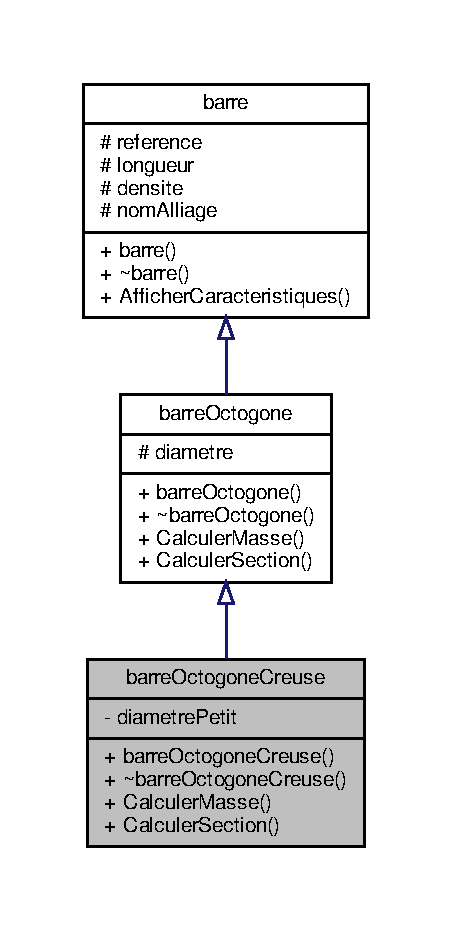
\includegraphics[width=217pt]{classbarre_octogone_creuse__inherit__graph}
\end{center}
\end{figure}


Graphe de collaboration de barre\+Octogone\+Creuse\+:
\nopagebreak
\begin{figure}[H]
\begin{center}
\leavevmode
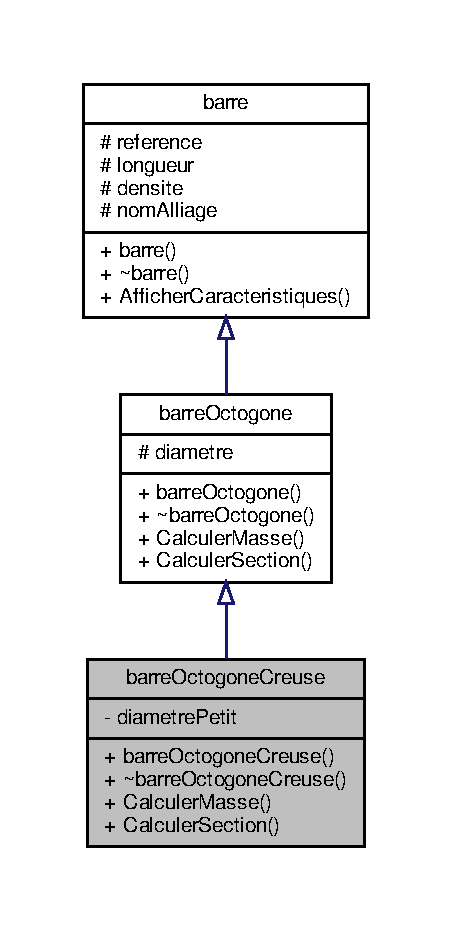
\includegraphics[width=217pt]{classbarre_octogone_creuse__coll__graph}
\end{center}
\end{figure}
\subsection*{Fonctions membres publiques}
\begin{DoxyCompactItemize}
\item 
\hyperlink{classbarre_octogone_creuse_a87882baf89e869f37c32d1cd27d62f43}{barre\+Octogone\+Creuse} (const string \+\_\+reference, const int \+\_\+longueur, const float \+\_\+densite, const string \+\_\+nom\+Alliage, const double \+\_\+diametre, const double \+\_\+diametre\+Petit)
\begin{DoxyCompactList}\small\item\em \hyperlink{classbarre_octogone_creuse_a87882baf89e869f37c32d1cd27d62f43}{barre\+Octogone\+Creuse\+::barre\+Octogone\+Creuse} \end{DoxyCompactList}\item 
\hyperlink{classbarre_octogone_creuse_aa93c0a16e1ccbcabb788f4c93ab7e7c9}{$\sim$barre\+Octogone\+Creuse} ()
\begin{DoxyCompactList}\small\item\em \hyperlink{classbarre_octogone_creuse_aa93c0a16e1ccbcabb788f4c93ab7e7c9}{barre\+Octogone\+Creuse\+::$\sim$barre\+Octogone\+Creuse} \end{DoxyCompactList}\item 
double \hyperlink{classbarre_octogone_creuse_a301de4f326c5e74317f640663f0dffc2}{Calculer\+Masse} ()
\begin{DoxyCompactList}\small\item\em \hyperlink{classbarre_octogone_creuse_a301de4f326c5e74317f640663f0dffc2}{barre\+Octogone\+Creuse\+::\+Calculer\+Masse} \end{DoxyCompactList}\item 
double \hyperlink{classbarre_octogone_creuse_a271dcf37a8794ec979ab82f87f99e218}{Calculer\+Section} ()
\begin{DoxyCompactList}\small\item\em \hyperlink{classbarre_octogone_creuse_a271dcf37a8794ec979ab82f87f99e218}{barre\+Octogone\+Creuse\+::\+Calculer\+Section} \end{DoxyCompactList}\end{DoxyCompactItemize}
\subsection*{Attributs privés}
\begin{DoxyCompactItemize}
\item 
double \hyperlink{classbarre_octogone_creuse_a6ce90d417e09ed69d6d4243e8bff355a}{diametre\+Petit}
\end{DoxyCompactItemize}
\subsection*{Membres hérités additionnels}


\subsection{Description détaillée}
The \hyperlink{classbarre_octogone_creuse}{barre\+Octogone\+Creuse} class. 

Definition de la classe Barre Octogone Creuse 

\subsection{Documentation des constructeurs et destructeur}
\mbox{\Hypertarget{classbarre_octogone_creuse_a87882baf89e869f37c32d1cd27d62f43}\label{classbarre_octogone_creuse_a87882baf89e869f37c32d1cd27d62f43}} 
\index{barre\+Octogone\+Creuse@{barre\+Octogone\+Creuse}!barre\+Octogone\+Creuse@{barre\+Octogone\+Creuse}}
\index{barre\+Octogone\+Creuse@{barre\+Octogone\+Creuse}!barre\+Octogone\+Creuse@{barre\+Octogone\+Creuse}}
\subsubsection{\texorpdfstring{barre\+Octogone\+Creuse()}{barreOctogoneCreuse()}}
{\footnotesize\ttfamily barre\+Octogone\+Creuse\+::barre\+Octogone\+Creuse (\begin{DoxyParamCaption}\item[{const string}]{\+\_\+reference,  }\item[{const int}]{\+\_\+longueur,  }\item[{const float}]{\+\_\+densite,  }\item[{const string}]{\+\_\+nom\+Alliage,  }\item[{const double}]{\+\_\+diametre,  }\item[{const double}]{\+\_\+diametre\+Petit }\end{DoxyParamCaption})}



\hyperlink{classbarre_octogone_creuse_a87882baf89e869f37c32d1cd27d62f43}{barre\+Octogone\+Creuse\+::barre\+Octogone\+Creuse} 


\begin{DoxyParams}{Paramètres}
{\em \+\_\+reference} & \\
\hline
{\em \+\_\+longueur} & \\
\hline
{\em \+\_\+densite} & \\
\hline
{\em \+\_\+nom\+Alliage} & \\
\hline
{\em \+\_\+diametre} & \\
\hline
{\em \+\_\+diametre\+Petit} & \\
\hline
\end{DoxyParams}
Constructeur de la classe Barre\+Octogone\+Creuse qui initialise ses parametres \mbox{\Hypertarget{classbarre_octogone_creuse_aa93c0a16e1ccbcabb788f4c93ab7e7c9}\label{classbarre_octogone_creuse_aa93c0a16e1ccbcabb788f4c93ab7e7c9}} 
\index{barre\+Octogone\+Creuse@{barre\+Octogone\+Creuse}!````~barre\+Octogone\+Creuse@{$\sim$barre\+Octogone\+Creuse}}
\index{````~barre\+Octogone\+Creuse@{$\sim$barre\+Octogone\+Creuse}!barre\+Octogone\+Creuse@{barre\+Octogone\+Creuse}}
\subsubsection{\texorpdfstring{$\sim$barre\+Octogone\+Creuse()}{~barreOctogoneCreuse()}}
{\footnotesize\ttfamily barre\+Octogone\+Creuse\+::$\sim$barre\+Octogone\+Creuse (\begin{DoxyParamCaption}{ }\end{DoxyParamCaption})}



\hyperlink{classbarre_octogone_creuse_aa93c0a16e1ccbcabb788f4c93ab7e7c9}{barre\+Octogone\+Creuse\+::$\sim$barre\+Octogone\+Creuse} 

Destructeur de la classe Barre\+Octogone\+Creuse 

\subsection{Documentation des fonctions membres}
\mbox{\Hypertarget{classbarre_octogone_creuse_a301de4f326c5e74317f640663f0dffc2}\label{classbarre_octogone_creuse_a301de4f326c5e74317f640663f0dffc2}} 
\index{barre\+Octogone\+Creuse@{barre\+Octogone\+Creuse}!Calculer\+Masse@{Calculer\+Masse}}
\index{Calculer\+Masse@{Calculer\+Masse}!barre\+Octogone\+Creuse@{barre\+Octogone\+Creuse}}
\subsubsection{\texorpdfstring{Calculer\+Masse()}{CalculerMasse()}}
{\footnotesize\ttfamily double barre\+Octogone\+Creuse\+::\+Calculer\+Masse (\begin{DoxyParamCaption}{ }\end{DoxyParamCaption})}



\hyperlink{classbarre_octogone_creuse_a301de4f326c5e74317f640663f0dffc2}{barre\+Octogone\+Creuse\+::\+Calculer\+Masse} 

\begin{DoxyReturn}{Renvoie}

\end{DoxyReturn}
Methode Calculer\+Masse qui renvoie la Masse \mbox{\Hypertarget{classbarre_octogone_creuse_a271dcf37a8794ec979ab82f87f99e218}\label{classbarre_octogone_creuse_a271dcf37a8794ec979ab82f87f99e218}} 
\index{barre\+Octogone\+Creuse@{barre\+Octogone\+Creuse}!Calculer\+Section@{Calculer\+Section}}
\index{Calculer\+Section@{Calculer\+Section}!barre\+Octogone\+Creuse@{barre\+Octogone\+Creuse}}
\subsubsection{\texorpdfstring{Calculer\+Section()}{CalculerSection()}}
{\footnotesize\ttfamily double barre\+Octogone\+Creuse\+::\+Calculer\+Section (\begin{DoxyParamCaption}{ }\end{DoxyParamCaption})}



\hyperlink{classbarre_octogone_creuse_a271dcf37a8794ec979ab82f87f99e218}{barre\+Octogone\+Creuse\+::\+Calculer\+Section} 

\begin{DoxyReturn}{Renvoie}

\end{DoxyReturn}
Methode Calculer\+Section qui renvoie la section de la barre creuse 

\subsection{Documentation des données membres}
\mbox{\Hypertarget{classbarre_octogone_creuse_a6ce90d417e09ed69d6d4243e8bff355a}\label{classbarre_octogone_creuse_a6ce90d417e09ed69d6d4243e8bff355a}} 
\index{barre\+Octogone\+Creuse@{barre\+Octogone\+Creuse}!diametre\+Petit@{diametre\+Petit}}
\index{diametre\+Petit@{diametre\+Petit}!barre\+Octogone\+Creuse@{barre\+Octogone\+Creuse}}
\subsubsection{\texorpdfstring{diametre\+Petit}{diametrePetit}}
{\footnotesize\ttfamily double barre\+Octogone\+Creuse\+::diametre\+Petit\hspace{0.3cm}{\ttfamily [private]}}



La documentation de cette classe a été générée à partir des fichiers suivants \+:\begin{DoxyCompactItemize}
\item 
T\+D\+\_\+\+Barre/\hyperlink{barreoctogonecreuse_8h}{barreoctogonecreuse.\+h}\item 
T\+D\+\_\+\+Barre/\hyperlink{barreoctogonecreuse_8cpp}{barreoctogonecreuse.\+cpp}\end{DoxyCompactItemize}

\hypertarget{classbarre_rectangle}{}\section{Référence de la classe barre\+Rectangle}
\label{classbarre_rectangle}\index{barre\+Rectangle@{barre\+Rectangle}}


The \hyperlink{classbarre_rectangle}{barre\+Rectangle} class.  




{\ttfamily \#include $<$barrerectangle.\+h$>$}



Graphe d\textquotesingle{}héritage de barre\+Rectangle\+:
\nopagebreak
\begin{figure}[H]
\begin{center}
\leavevmode
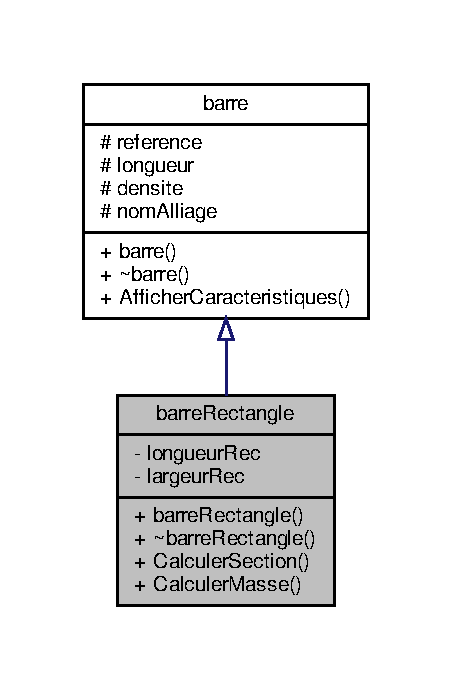
\includegraphics[width=217pt]{classbarre_rectangle__inherit__graph}
\end{center}
\end{figure}


Graphe de collaboration de barre\+Rectangle\+:
\nopagebreak
\begin{figure}[H]
\begin{center}
\leavevmode
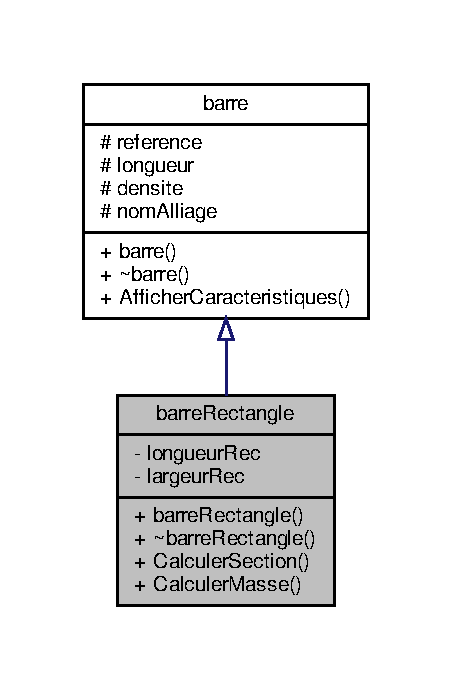
\includegraphics[width=217pt]{classbarre_rectangle__coll__graph}
\end{center}
\end{figure}
\subsection*{Fonctions membres publiques}
\begin{DoxyCompactItemize}
\item 
\hyperlink{classbarre_rectangle_a3d5270d95f3ee2c6d4074495f7fd9859}{barre\+Rectangle} (const string \+\_\+reference, const int \+\_\+longueur, const float \+\_\+densite, const string \+\_\+nom\+Alliage, const int \+\_\+longueur\+Rec, const int \+\_\+largeur\+Rec)
\begin{DoxyCompactList}\small\item\em \hyperlink{classbarre_rectangle_a3d5270d95f3ee2c6d4074495f7fd9859}{barre\+Rectangle\+::barre\+Rectangle} \end{DoxyCompactList}\item 
\hyperlink{classbarre_rectangle_a27c21df460fbde7f24ac2a7540558091}{$\sim$barre\+Rectangle} ()
\begin{DoxyCompactList}\small\item\em \hyperlink{classbarre_rectangle_a27c21df460fbde7f24ac2a7540558091}{barre\+Rectangle\+::$\sim$barre\+Rectangle} \end{DoxyCompactList}\item 
double \hyperlink{classbarre_rectangle_a321e3526a980b5d48a5cf9a05ee2b63a}{Calculer\+Section} ()
\begin{DoxyCompactList}\small\item\em \hyperlink{classbarre_rectangle_a321e3526a980b5d48a5cf9a05ee2b63a}{barre\+Rectangle\+::\+Calculer\+Section} \end{DoxyCompactList}\item 
double \hyperlink{classbarre_rectangle_ac558660f43d5e18472aaa57ee98d5fd0}{Calculer\+Masse} ()
\begin{DoxyCompactList}\small\item\em \hyperlink{classbarre_rectangle_ac558660f43d5e18472aaa57ee98d5fd0}{barre\+Rectangle\+::\+Calculer\+Masse} \end{DoxyCompactList}\end{DoxyCompactItemize}
\subsection*{Attributs privés}
\begin{DoxyCompactItemize}
\item 
int \hyperlink{classbarre_rectangle_a5df869c01c9a2e2dad98fa392fa59c85}{longueur\+Rec}
\item 
int \hyperlink{classbarre_rectangle_a9420b90a6b3d44b807ca716abae6039e}{largeur\+Rec}
\end{DoxyCompactItemize}
\subsection*{Membres hérités additionnels}


\subsection{Description détaillée}
The \hyperlink{classbarre_rectangle}{barre\+Rectangle} class. 

Definition de la classe \hyperlink{classbarre_rectangle}{barre\+Rectangle} qui herite de barre 

\subsection{Documentation des constructeurs et destructeur}
\mbox{\Hypertarget{classbarre_rectangle_a3d5270d95f3ee2c6d4074495f7fd9859}\label{classbarre_rectangle_a3d5270d95f3ee2c6d4074495f7fd9859}} 
\index{barre\+Rectangle@{barre\+Rectangle}!barre\+Rectangle@{barre\+Rectangle}}
\index{barre\+Rectangle@{barre\+Rectangle}!barre\+Rectangle@{barre\+Rectangle}}
\subsubsection{\texorpdfstring{barre\+Rectangle()}{barreRectangle()}}
{\footnotesize\ttfamily barre\+Rectangle\+::barre\+Rectangle (\begin{DoxyParamCaption}\item[{const string}]{\+\_\+reference,  }\item[{const int}]{\+\_\+longueur,  }\item[{const float}]{\+\_\+densite,  }\item[{const string}]{\+\_\+nom\+Alliage,  }\item[{const int}]{\+\_\+longueur\+Rec,  }\item[{const int}]{\+\_\+largeur\+Rec }\end{DoxyParamCaption})}



\hyperlink{classbarre_rectangle_a3d5270d95f3ee2c6d4074495f7fd9859}{barre\+Rectangle\+::barre\+Rectangle} 


\begin{DoxyParams}{Paramètres}
{\em \+\_\+reference} & \\
\hline
{\em \+\_\+longueur} & \\
\hline
{\em \+\_\+densite} & \\
\hline
{\em \+\_\+nom\+Alliage} & \\
\hline
{\em \+\_\+longueur\+Rec} & \\
\hline
{\em \+\_\+largeur\+Rec} & \\
\hline
\end{DoxyParams}
Constructeur de la classe \hyperlink{classbarre_rectangle}{barre\+Rectangle} qui initialise les parametres \mbox{\Hypertarget{classbarre_rectangle_a27c21df460fbde7f24ac2a7540558091}\label{classbarre_rectangle_a27c21df460fbde7f24ac2a7540558091}} 
\index{barre\+Rectangle@{barre\+Rectangle}!````~barre\+Rectangle@{$\sim$barre\+Rectangle}}
\index{````~barre\+Rectangle@{$\sim$barre\+Rectangle}!barre\+Rectangle@{barre\+Rectangle}}
\subsubsection{\texorpdfstring{$\sim$barre\+Rectangle()}{~barreRectangle()}}
{\footnotesize\ttfamily barre\+Rectangle\+::$\sim$barre\+Rectangle (\begin{DoxyParamCaption}{ }\end{DoxyParamCaption})}



\hyperlink{classbarre_rectangle_a27c21df460fbde7f24ac2a7540558091}{barre\+Rectangle\+::$\sim$barre\+Rectangle} 

Destructeur de la classe Barre\+Rectangle 

\subsection{Documentation des fonctions membres}
\mbox{\Hypertarget{classbarre_rectangle_ac558660f43d5e18472aaa57ee98d5fd0}\label{classbarre_rectangle_ac558660f43d5e18472aaa57ee98d5fd0}} 
\index{barre\+Rectangle@{barre\+Rectangle}!Calculer\+Masse@{Calculer\+Masse}}
\index{Calculer\+Masse@{Calculer\+Masse}!barre\+Rectangle@{barre\+Rectangle}}
\subsubsection{\texorpdfstring{Calculer\+Masse()}{CalculerMasse()}}
{\footnotesize\ttfamily double barre\+Rectangle\+::\+Calculer\+Masse (\begin{DoxyParamCaption}{ }\end{DoxyParamCaption})}



\hyperlink{classbarre_rectangle_ac558660f43d5e18472aaa57ee98d5fd0}{barre\+Rectangle\+::\+Calculer\+Masse} 

\begin{DoxyReturn}{Renvoie}

\end{DoxyReturn}
Methode Calculer\+Masse qui renvoie la masse \mbox{\Hypertarget{classbarre_rectangle_a321e3526a980b5d48a5cf9a05ee2b63a}\label{classbarre_rectangle_a321e3526a980b5d48a5cf9a05ee2b63a}} 
\index{barre\+Rectangle@{barre\+Rectangle}!Calculer\+Section@{Calculer\+Section}}
\index{Calculer\+Section@{Calculer\+Section}!barre\+Rectangle@{barre\+Rectangle}}
\subsubsection{\texorpdfstring{Calculer\+Section()}{CalculerSection()}}
{\footnotesize\ttfamily double barre\+Rectangle\+::\+Calculer\+Section (\begin{DoxyParamCaption}{ }\end{DoxyParamCaption})}



\hyperlink{classbarre_rectangle_a321e3526a980b5d48a5cf9a05ee2b63a}{barre\+Rectangle\+::\+Calculer\+Section} 

Methode Calculer\+Section qui renvoie la section \begin{DoxyReturn}{Renvoie}

\end{DoxyReturn}


\subsection{Documentation des données membres}
\mbox{\Hypertarget{classbarre_rectangle_a9420b90a6b3d44b807ca716abae6039e}\label{classbarre_rectangle_a9420b90a6b3d44b807ca716abae6039e}} 
\index{barre\+Rectangle@{barre\+Rectangle}!largeur\+Rec@{largeur\+Rec}}
\index{largeur\+Rec@{largeur\+Rec}!barre\+Rectangle@{barre\+Rectangle}}
\subsubsection{\texorpdfstring{largeur\+Rec}{largeurRec}}
{\footnotesize\ttfamily int barre\+Rectangle\+::largeur\+Rec\hspace{0.3cm}{\ttfamily [private]}}

\mbox{\Hypertarget{classbarre_rectangle_a5df869c01c9a2e2dad98fa392fa59c85}\label{classbarre_rectangle_a5df869c01c9a2e2dad98fa392fa59c85}} 
\index{barre\+Rectangle@{barre\+Rectangle}!longueur\+Rec@{longueur\+Rec}}
\index{longueur\+Rec@{longueur\+Rec}!barre\+Rectangle@{barre\+Rectangle}}
\subsubsection{\texorpdfstring{longueur\+Rec}{longueurRec}}
{\footnotesize\ttfamily int barre\+Rectangle\+::longueur\+Rec\hspace{0.3cm}{\ttfamily [private]}}



La documentation de cette classe a été générée à partir des fichiers suivants \+:\begin{DoxyCompactItemize}
\item 
T\+D\+\_\+\+Barre/\hyperlink{barrerectangle_8h}{barrerectangle.\+h}\item 
T\+D\+\_\+\+Barre/\hyperlink{barrerectangle_8cpp}{barrerectangle.\+cpp}\end{DoxyCompactItemize}

\hypertarget{classbarre_ronde}{}\section{Référence de la classe barre\+Ronde}
\label{classbarre_ronde}\index{barre\+Ronde@{barre\+Ronde}}


The \hyperlink{classbarre_ronde}{barre\+Ronde} class.  




{\ttfamily \#include $<$barreronde.\+h$>$}



Graphe d\textquotesingle{}héritage de barre\+Ronde\+:
\nopagebreak
\begin{figure}[H]
\begin{center}
\leavevmode
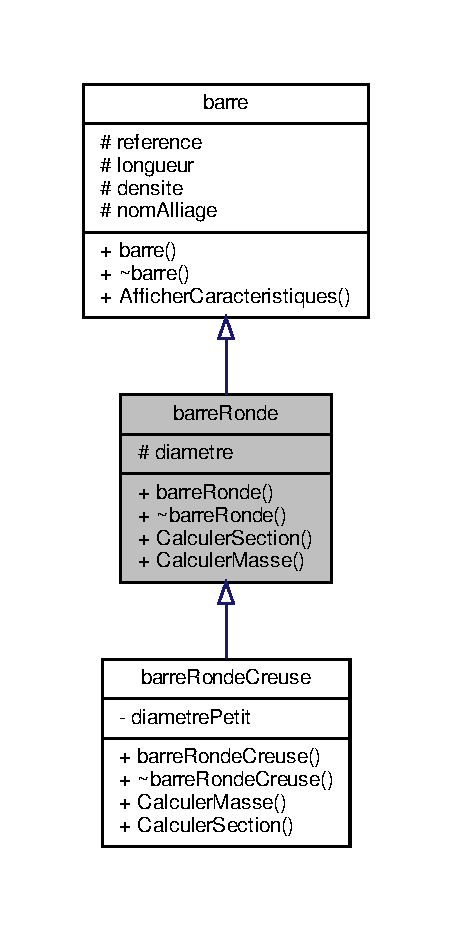
\includegraphics[width=217pt]{classbarre_ronde__inherit__graph}
\end{center}
\end{figure}


Graphe de collaboration de barre\+Ronde\+:
\nopagebreak
\begin{figure}[H]
\begin{center}
\leavevmode
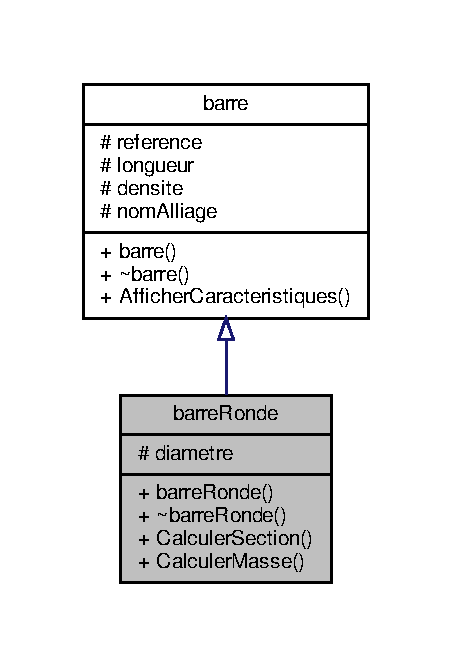
\includegraphics[width=217pt]{classbarre_ronde__coll__graph}
\end{center}
\end{figure}
\subsection*{Fonctions membres publiques}
\begin{DoxyCompactItemize}
\item 
\hyperlink{classbarre_ronde_afde29e31ebfa5236624fb74205cdc487}{barre\+Ronde} (const string \+\_\+reference, const int \+\_\+longueur, const float \+\_\+densite, const string \+\_\+nom\+Alliage, const double \hyperlink{classbarre_ronde_a351f886cdb9bd89132c1ae839f1e9f2e}{diametre})
\begin{DoxyCompactList}\small\item\em \hyperlink{classbarre_ronde_afde29e31ebfa5236624fb74205cdc487}{barre\+Ronde\+::barre\+Ronde} \end{DoxyCompactList}\item 
\hyperlink{classbarre_ronde_ad297441fd7476ed15d45dc0030207125}{$\sim$barre\+Ronde} ()
\begin{DoxyCompactList}\small\item\em \hyperlink{classbarre_ronde_ad297441fd7476ed15d45dc0030207125}{barre\+Ronde\+::$\sim$barre\+Ronde} \end{DoxyCompactList}\item 
double \hyperlink{classbarre_ronde_aab6bddac0a3e8b9eb43d35903f5b4bc4}{Calculer\+Section} ()
\begin{DoxyCompactList}\small\item\em \hyperlink{classbarre_ronde_aab6bddac0a3e8b9eb43d35903f5b4bc4}{barre\+Ronde\+::\+Calculer\+Section} \end{DoxyCompactList}\item 
double \hyperlink{classbarre_ronde_aca5b7e7ce02356570eb86d048788e076}{Calculer\+Masse} ()
\begin{DoxyCompactList}\small\item\em \hyperlink{classbarre_ronde_aca5b7e7ce02356570eb86d048788e076}{barre\+Ronde\+::\+Calculer\+Masse} \end{DoxyCompactList}\end{DoxyCompactItemize}
\subsection*{Attributs protégés}
\begin{DoxyCompactItemize}
\item 
double \hyperlink{classbarre_ronde_a351f886cdb9bd89132c1ae839f1e9f2e}{diametre}
\end{DoxyCompactItemize}


\subsection{Description détaillée}
The \hyperlink{classbarre_ronde}{barre\+Ronde} class. 

definition de la classe Barre\+Ronde qui herite de barre 

\subsection{Documentation des constructeurs et destructeur}
\mbox{\Hypertarget{classbarre_ronde_afde29e31ebfa5236624fb74205cdc487}\label{classbarre_ronde_afde29e31ebfa5236624fb74205cdc487}} 
\index{barre\+Ronde@{barre\+Ronde}!barre\+Ronde@{barre\+Ronde}}
\index{barre\+Ronde@{barre\+Ronde}!barre\+Ronde@{barre\+Ronde}}
\subsubsection{\texorpdfstring{barre\+Ronde()}{barreRonde()}}
{\footnotesize\ttfamily barre\+Ronde\+::barre\+Ronde (\begin{DoxyParamCaption}\item[{const string}]{\+\_\+reference,  }\item[{const int}]{\+\_\+longueur,  }\item[{const float}]{\+\_\+densite,  }\item[{const string}]{\+\_\+nom\+Alliage,  }\item[{const double}]{\+\_\+diametre }\end{DoxyParamCaption})}



\hyperlink{classbarre_ronde_afde29e31ebfa5236624fb74205cdc487}{barre\+Ronde\+::barre\+Ronde} 


\begin{DoxyParams}{Paramètres}
{\em \+\_\+reference} & \\
\hline
{\em \+\_\+longueur} & \\
\hline
{\em \+\_\+densite} & \\
\hline
{\em \+\_\+nom\+Alliage} & \\
\hline
{\em \+\_\+diametre} & \\
\hline
\end{DoxyParams}
Contructeur de la Classe Barre\+Ronde qui initialise les parametres \mbox{\Hypertarget{classbarre_ronde_ad297441fd7476ed15d45dc0030207125}\label{classbarre_ronde_ad297441fd7476ed15d45dc0030207125}} 
\index{barre\+Ronde@{barre\+Ronde}!````~barre\+Ronde@{$\sim$barre\+Ronde}}
\index{````~barre\+Ronde@{$\sim$barre\+Ronde}!barre\+Ronde@{barre\+Ronde}}
\subsubsection{\texorpdfstring{$\sim$barre\+Ronde()}{~barreRonde()}}
{\footnotesize\ttfamily barre\+Ronde\+::$\sim$barre\+Ronde (\begin{DoxyParamCaption}{ }\end{DoxyParamCaption})}



\hyperlink{classbarre_ronde_ad297441fd7476ed15d45dc0030207125}{barre\+Ronde\+::$\sim$barre\+Ronde} 

Destructeur de la classe Barre\+Ronde 

\subsection{Documentation des fonctions membres}
\mbox{\Hypertarget{classbarre_ronde_aca5b7e7ce02356570eb86d048788e076}\label{classbarre_ronde_aca5b7e7ce02356570eb86d048788e076}} 
\index{barre\+Ronde@{barre\+Ronde}!Calculer\+Masse@{Calculer\+Masse}}
\index{Calculer\+Masse@{Calculer\+Masse}!barre\+Ronde@{barre\+Ronde}}
\subsubsection{\texorpdfstring{Calculer\+Masse()}{CalculerMasse()}}
{\footnotesize\ttfamily double barre\+Ronde\+::\+Calculer\+Masse (\begin{DoxyParamCaption}{ }\end{DoxyParamCaption})}



\hyperlink{classbarre_ronde_aca5b7e7ce02356570eb86d048788e076}{barre\+Ronde\+::\+Calculer\+Masse} 

Methode Calculer\+Masse qui renvoie la masse de l\textquotesingle{}objet \begin{DoxyReturn}{Renvoie}

\end{DoxyReturn}
On change le type de longueur et densite en double \mbox{\Hypertarget{classbarre_ronde_aab6bddac0a3e8b9eb43d35903f5b4bc4}\label{classbarre_ronde_aab6bddac0a3e8b9eb43d35903f5b4bc4}} 
\index{barre\+Ronde@{barre\+Ronde}!Calculer\+Section@{Calculer\+Section}}
\index{Calculer\+Section@{Calculer\+Section}!barre\+Ronde@{barre\+Ronde}}
\subsubsection{\texorpdfstring{Calculer\+Section()}{CalculerSection()}}
{\footnotesize\ttfamily double barre\+Ronde\+::\+Calculer\+Section (\begin{DoxyParamCaption}{ }\end{DoxyParamCaption})}



\hyperlink{classbarre_ronde_aab6bddac0a3e8b9eb43d35903f5b4bc4}{barre\+Ronde\+::\+Calculer\+Section} 

Methode Calculer\+Section qui renvoie la section de l\textquotesingle{}objet \begin{DoxyReturn}{Renvoie}

\end{DoxyReturn}


\subsection{Documentation des données membres}
\mbox{\Hypertarget{classbarre_ronde_a351f886cdb9bd89132c1ae839f1e9f2e}\label{classbarre_ronde_a351f886cdb9bd89132c1ae839f1e9f2e}} 
\index{barre\+Ronde@{barre\+Ronde}!diametre@{diametre}}
\index{diametre@{diametre}!barre\+Ronde@{barre\+Ronde}}
\subsubsection{\texorpdfstring{diametre}{diametre}}
{\footnotesize\ttfamily double barre\+Ronde\+::diametre\hspace{0.3cm}{\ttfamily [protected]}}



La documentation de cette classe a été générée à partir des fichiers suivants \+:\begin{DoxyCompactItemize}
\item 
T\+D\+\_\+\+Barre/\hyperlink{barreronde_8h}{barreronde.\+h}\item 
T\+D\+\_\+\+Barre/\hyperlink{barreronde_8cpp}{barreronde.\+cpp}\end{DoxyCompactItemize}

\hypertarget{classbarre_ronde_creuse}{}\section{Référence de la classe barre\+Ronde\+Creuse}
\label{classbarre_ronde_creuse}\index{barre\+Ronde\+Creuse@{barre\+Ronde\+Creuse}}


The \hyperlink{classbarre_ronde_creuse}{barre\+Ronde\+Creuse} class.  




{\ttfamily \#include $<$barrerondecreuse.\+h$>$}



Graphe d\textquotesingle{}héritage de barre\+Ronde\+Creuse\+:
\nopagebreak
\begin{figure}[H]
\begin{center}
\leavevmode
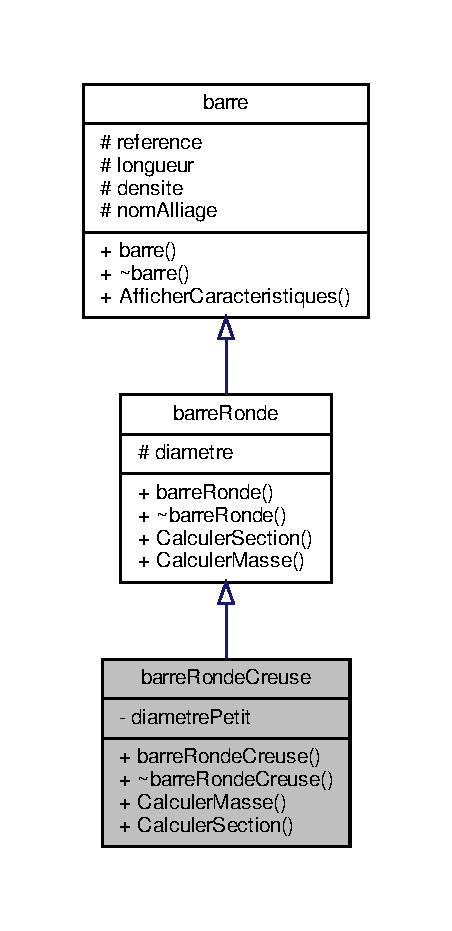
\includegraphics[width=217pt]{classbarre_ronde_creuse__inherit__graph}
\end{center}
\end{figure}


Graphe de collaboration de barre\+Ronde\+Creuse\+:
\nopagebreak
\begin{figure}[H]
\begin{center}
\leavevmode
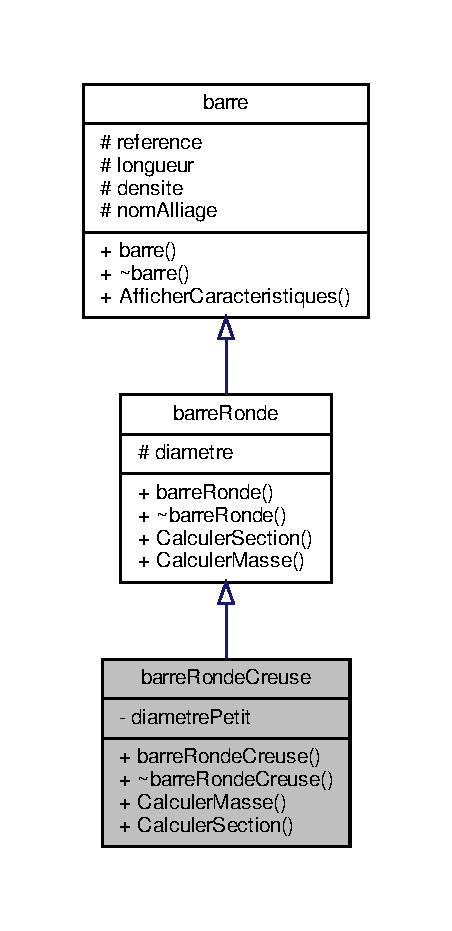
\includegraphics[width=217pt]{classbarre_ronde_creuse__coll__graph}
\end{center}
\end{figure}
\subsection*{Fonctions membres publiques}
\begin{DoxyCompactItemize}
\item 
\hyperlink{classbarre_ronde_creuse_aa3b1bff9d23a8f5740f082684aec2956}{barre\+Ronde\+Creuse} (const string \+\_\+reference, const int \+\_\+longueur, const float \+\_\+densite, const string \+\_\+nom\+Alliage, const double \+\_\+diametre, const double \+\_\+diametre\+Petit)
\begin{DoxyCompactList}\small\item\em \hyperlink{classbarre_ronde_creuse_aa3b1bff9d23a8f5740f082684aec2956}{barre\+Ronde\+Creuse\+::barre\+Ronde\+Creuse} \end{DoxyCompactList}\item 
\hyperlink{classbarre_ronde_creuse_aec4dfe7298ca1b2885e7f090fbb94954}{$\sim$barre\+Ronde\+Creuse} ()
\begin{DoxyCompactList}\small\item\em \hyperlink{classbarre_ronde_creuse_aec4dfe7298ca1b2885e7f090fbb94954}{barre\+Ronde\+Creuse\+::$\sim$barre\+Ronde\+Creuse} \end{DoxyCompactList}\item 
double \hyperlink{classbarre_ronde_creuse_a5c6242830085be53d968cb23602ea2b1}{Calculer\+Masse} ()
\begin{DoxyCompactList}\small\item\em \hyperlink{classbarre_ronde_creuse_a5c6242830085be53d968cb23602ea2b1}{barre\+Ronde\+Creuse\+::\+Calculer\+Masse} \end{DoxyCompactList}\item 
double \hyperlink{classbarre_ronde_creuse_adbd7d165624ef3580e7c85cd777cd95f}{Calculer\+Section} ()
\begin{DoxyCompactList}\small\item\em \hyperlink{classbarre_ronde_creuse_adbd7d165624ef3580e7c85cd777cd95f}{barre\+Ronde\+Creuse\+::\+Calculer\+Section} \end{DoxyCompactList}\end{DoxyCompactItemize}
\subsection*{Attributs privés}
\begin{DoxyCompactItemize}
\item 
double \hyperlink{classbarre_ronde_creuse_a78869588e151b3b0e3b1938eb8ebd0a0}{diametre\+Petit}
\end{DoxyCompactItemize}
\subsection*{Membres hérités additionnels}


\subsection{Description détaillée}
The \hyperlink{classbarre_ronde_creuse}{barre\+Ronde\+Creuse} class. 

definition de la Classe Barre\+Ronde\+Creuse qui herite de \hyperlink{classbarre_ronde}{barre\+Ronde} 

\subsection{Documentation des constructeurs et destructeur}
\mbox{\Hypertarget{classbarre_ronde_creuse_aa3b1bff9d23a8f5740f082684aec2956}\label{classbarre_ronde_creuse_aa3b1bff9d23a8f5740f082684aec2956}} 
\index{barre\+Ronde\+Creuse@{barre\+Ronde\+Creuse}!barre\+Ronde\+Creuse@{barre\+Ronde\+Creuse}}
\index{barre\+Ronde\+Creuse@{barre\+Ronde\+Creuse}!barre\+Ronde\+Creuse@{barre\+Ronde\+Creuse}}
\subsubsection{\texorpdfstring{barre\+Ronde\+Creuse()}{barreRondeCreuse()}}
{\footnotesize\ttfamily barre\+Ronde\+Creuse\+::barre\+Ronde\+Creuse (\begin{DoxyParamCaption}\item[{const string}]{\+\_\+reference,  }\item[{const int}]{\+\_\+longueur,  }\item[{const float}]{\+\_\+densite,  }\item[{const string}]{\+\_\+nom\+Alliage,  }\item[{const double}]{\+\_\+diametre,  }\item[{const double}]{\+\_\+diametre\+Petit }\end{DoxyParamCaption})}



\hyperlink{classbarre_ronde_creuse_aa3b1bff9d23a8f5740f082684aec2956}{barre\+Ronde\+Creuse\+::barre\+Ronde\+Creuse} 


\begin{DoxyParams}{Paramètres}
{\em \+\_\+reference} & \\
\hline
{\em \+\_\+longueur} & \\
\hline
{\em \+\_\+densite} & \\
\hline
{\em \+\_\+nom\+Alliage} & \\
\hline
{\em \+\_\+diametre} & \\
\hline
{\em \+\_\+diametre\+Petit} & \\
\hline
\end{DoxyParams}
Constructeur de la Classe Barre Ronde Creuse qui initialise les paramètres de la classe \mbox{\Hypertarget{classbarre_ronde_creuse_aec4dfe7298ca1b2885e7f090fbb94954}\label{classbarre_ronde_creuse_aec4dfe7298ca1b2885e7f090fbb94954}} 
\index{barre\+Ronde\+Creuse@{barre\+Ronde\+Creuse}!````~barre\+Ronde\+Creuse@{$\sim$barre\+Ronde\+Creuse}}
\index{````~barre\+Ronde\+Creuse@{$\sim$barre\+Ronde\+Creuse}!barre\+Ronde\+Creuse@{barre\+Ronde\+Creuse}}
\subsubsection{\texorpdfstring{$\sim$barre\+Ronde\+Creuse()}{~barreRondeCreuse()}}
{\footnotesize\ttfamily barre\+Ronde\+Creuse\+::$\sim$barre\+Ronde\+Creuse (\begin{DoxyParamCaption}{ }\end{DoxyParamCaption})}



\hyperlink{classbarre_ronde_creuse_aec4dfe7298ca1b2885e7f090fbb94954}{barre\+Ronde\+Creuse\+::$\sim$barre\+Ronde\+Creuse} 

Destructeur de la Classe Barre\+Ronde\+Creuse 

\subsection{Documentation des fonctions membres}
\mbox{\Hypertarget{classbarre_ronde_creuse_a5c6242830085be53d968cb23602ea2b1}\label{classbarre_ronde_creuse_a5c6242830085be53d968cb23602ea2b1}} 
\index{barre\+Ronde\+Creuse@{barre\+Ronde\+Creuse}!Calculer\+Masse@{Calculer\+Masse}}
\index{Calculer\+Masse@{Calculer\+Masse}!barre\+Ronde\+Creuse@{barre\+Ronde\+Creuse}}
\subsubsection{\texorpdfstring{Calculer\+Masse()}{CalculerMasse()}}
{\footnotesize\ttfamily double barre\+Ronde\+Creuse\+::\+Calculer\+Masse (\begin{DoxyParamCaption}{ }\end{DoxyParamCaption})}



\hyperlink{classbarre_ronde_creuse_a5c6242830085be53d968cb23602ea2b1}{barre\+Ronde\+Creuse\+::\+Calculer\+Masse} 

Methode Calculer\+Masse qui renvoie la Masse \begin{DoxyReturn}{Renvoie}

\end{DoxyReturn}
On transforme longueur et densite en double car masse est un double \mbox{\Hypertarget{classbarre_ronde_creuse_adbd7d165624ef3580e7c85cd777cd95f}\label{classbarre_ronde_creuse_adbd7d165624ef3580e7c85cd777cd95f}} 
\index{barre\+Ronde\+Creuse@{barre\+Ronde\+Creuse}!Calculer\+Section@{Calculer\+Section}}
\index{Calculer\+Section@{Calculer\+Section}!barre\+Ronde\+Creuse@{barre\+Ronde\+Creuse}}
\subsubsection{\texorpdfstring{Calculer\+Section()}{CalculerSection()}}
{\footnotesize\ttfamily double barre\+Ronde\+Creuse\+::\+Calculer\+Section (\begin{DoxyParamCaption}{ }\end{DoxyParamCaption})}



\hyperlink{classbarre_ronde_creuse_adbd7d165624ef3580e7c85cd777cd95f}{barre\+Ronde\+Creuse\+::\+Calculer\+Section} 

Methode Calculer\+Section qui renvoie la section Totale de l\textquotesingle{}objet \begin{DoxyReturn}{Renvoie}

\end{DoxyReturn}


\subsection{Documentation des données membres}
\mbox{\Hypertarget{classbarre_ronde_creuse_a78869588e151b3b0e3b1938eb8ebd0a0}\label{classbarre_ronde_creuse_a78869588e151b3b0e3b1938eb8ebd0a0}} 
\index{barre\+Ronde\+Creuse@{barre\+Ronde\+Creuse}!diametre\+Petit@{diametre\+Petit}}
\index{diametre\+Petit@{diametre\+Petit}!barre\+Ronde\+Creuse@{barre\+Ronde\+Creuse}}
\subsubsection{\texorpdfstring{diametre\+Petit}{diametrePetit}}
{\footnotesize\ttfamily double barre\+Ronde\+Creuse\+::diametre\+Petit\hspace{0.3cm}{\ttfamily [private]}}



La documentation de cette classe a été générée à partir des fichiers suivants \+:\begin{DoxyCompactItemize}
\item 
T\+D\+\_\+\+Barre/\hyperlink{barrerondecreuse_8h}{barrerondecreuse.\+h}\item 
T\+D\+\_\+\+Barre/\hyperlink{barrerondecreuse_8cpp}{barrerondecreuse.\+cpp}\end{DoxyCompactItemize}

\chapter{Documentation des fichiers}
\hypertarget{barre_8cpp}{}\section{Référence du fichier T\+D\+\_\+\+Barre/barre.cpp}
\label{barre_8cpp}\index{T\+D\+\_\+\+Barre/barre.\+cpp@{T\+D\+\_\+\+Barre/barre.\+cpp}}
{\ttfamily \#include \char`\"{}barre.\+h\char`\"{}}\newline
Graphe des dépendances par inclusion de barre.\+cpp\+:
\nopagebreak
\begin{figure}[H]
\begin{center}
\leavevmode
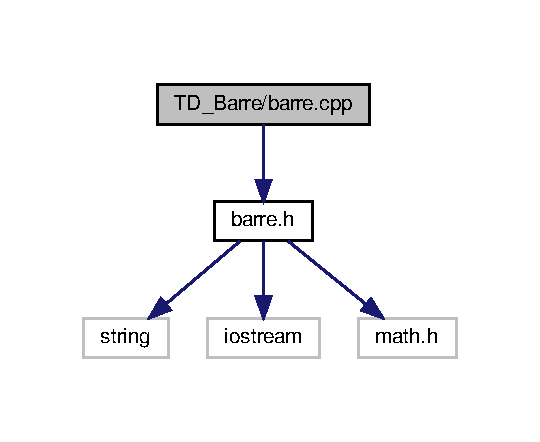
\includegraphics[width=259pt]{barre_8cpp__incl}
\end{center}
\end{figure}

\hypertarget{barre_8h}{}\section{Référence du fichier T\+D\+\_\+\+Barre/barre.h}
\label{barre_8h}\index{T\+D\+\_\+\+Barre/barre.\+h@{T\+D\+\_\+\+Barre/barre.\+h}}
{\ttfamily \#include $<$string$>$}\newline
{\ttfamily \#include $<$iostream$>$}\newline
{\ttfamily \#include $<$math.\+h$>$}\newline
Graphe des dépendances par inclusion de barre.\+h\+:
\nopagebreak
\begin{figure}[H]
\begin{center}
\leavevmode
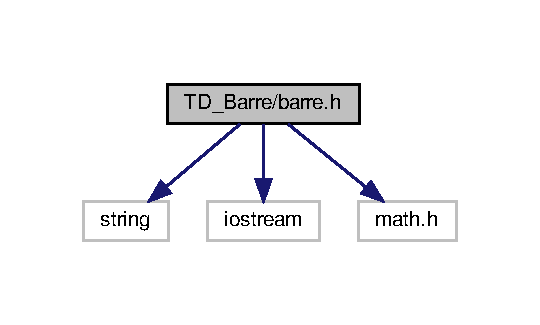
\includegraphics[width=259pt]{barre_8h__incl}
\end{center}
\end{figure}
Ce graphe montre quels fichiers incluent directement ou indirectement ce fichier \+:
\nopagebreak
\begin{figure}[H]
\begin{center}
\leavevmode
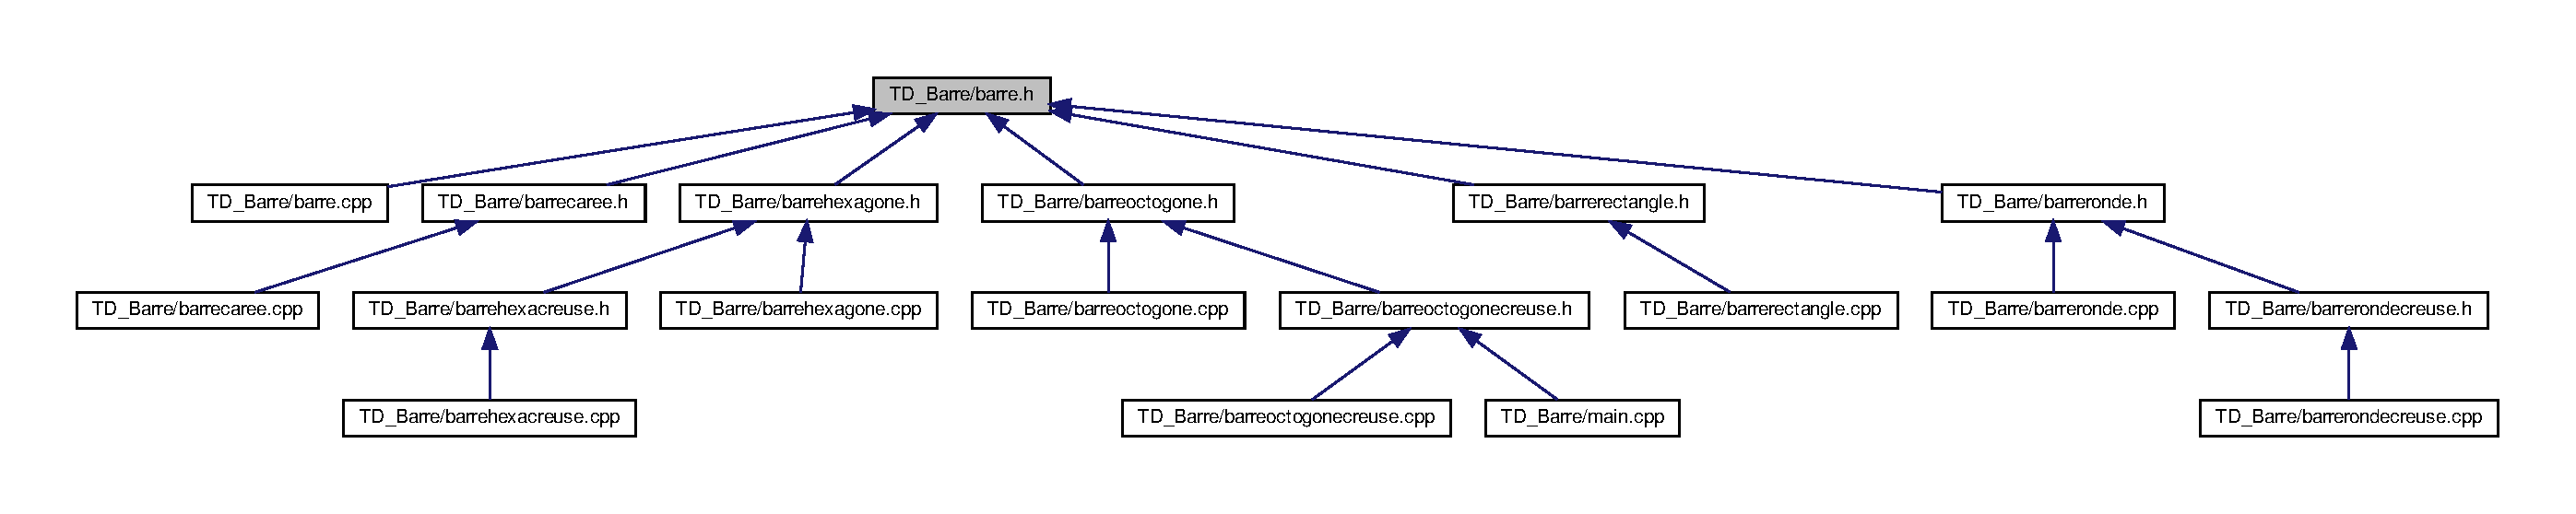
\includegraphics[width=350pt]{barre_8h__dep__incl}
\end{center}
\end{figure}
\subsection*{Classes}
\begin{DoxyCompactItemize}
\item 
class \hyperlink{classbarre}{barre}
\begin{DoxyCompactList}\small\item\em The barre class. \end{DoxyCompactList}\end{DoxyCompactItemize}

\hypertarget{barrecaree_8cpp}{}\section{Référence du fichier T\+D\+\_\+\+Barre/barrecaree.cpp}
\label{barrecaree_8cpp}\index{T\+D\+\_\+\+Barre/barrecaree.\+cpp@{T\+D\+\_\+\+Barre/barrecaree.\+cpp}}
{\ttfamily \#include \char`\"{}barrecaree.\+h\char`\"{}}\newline
Graphe des dépendances par inclusion de barrecaree.\+cpp\+:
\nopagebreak
\begin{figure}[H]
\begin{center}
\leavevmode
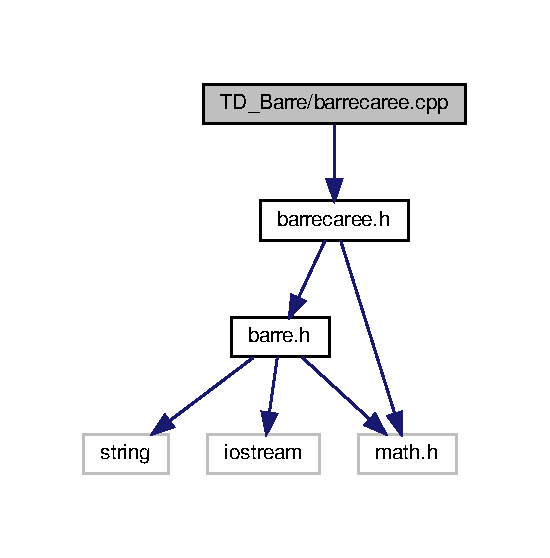
\includegraphics[width=264pt]{barrecaree_8cpp__incl}
\end{center}
\end{figure}

\hypertarget{barrecaree_8h}{}\section{Référence du fichier T\+D\+\_\+\+Barre/barrecaree.h}
\label{barrecaree_8h}\index{T\+D\+\_\+\+Barre/barrecaree.\+h@{T\+D\+\_\+\+Barre/barrecaree.\+h}}
{\ttfamily \#include \char`\"{}barre.\+h\char`\"{}}\newline
{\ttfamily \#include $<$math.\+h$>$}\newline
Graphe des dépendances par inclusion de barrecaree.\+h\+:
\nopagebreak
\begin{figure}[H]
\begin{center}
\leavevmode
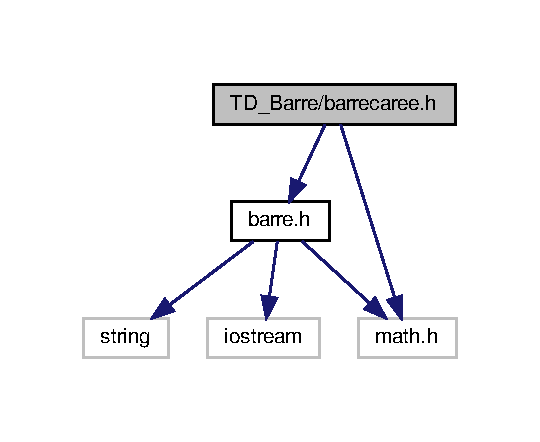
\includegraphics[width=259pt]{barrecaree_8h__incl}
\end{center}
\end{figure}
Ce graphe montre quels fichiers incluent directement ou indirectement ce fichier \+:
\nopagebreak
\begin{figure}[H]
\begin{center}
\leavevmode
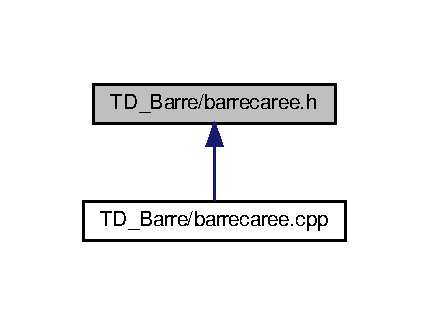
\includegraphics[width=206pt]{barrecaree_8h__dep__incl}
\end{center}
\end{figure}
\subsection*{Classes}
\begin{DoxyCompactItemize}
\item 
class \hyperlink{classbarre_carree}{barre\+Carree}
\begin{DoxyCompactList}\small\item\em The \hyperlink{classbarre_carree}{barre\+Carree} class. \end{DoxyCompactList}\end{DoxyCompactItemize}

\hypertarget{barrehexacreuse_8cpp}{}\section{Référence du fichier T\+D\+\_\+\+Barre/barrehexacreuse.cpp}
\label{barrehexacreuse_8cpp}\index{T\+D\+\_\+\+Barre/barrehexacreuse.\+cpp@{T\+D\+\_\+\+Barre/barrehexacreuse.\+cpp}}
{\ttfamily \#include \char`\"{}barrehexacreuse.\+h\char`\"{}}\newline
Graphe des dépendances par inclusion de barrehexacreuse.\+cpp\+:
\nopagebreak
\begin{figure}[H]
\begin{center}
\leavevmode
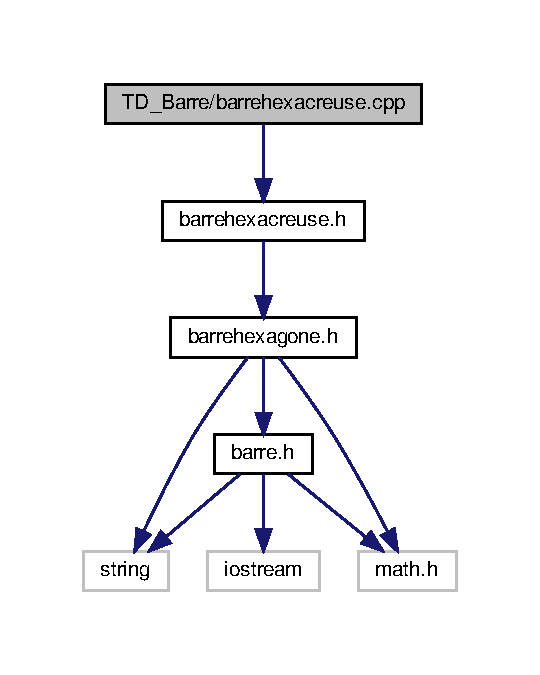
\includegraphics[width=259pt]{barrehexacreuse_8cpp__incl}
\end{center}
\end{figure}

\hypertarget{barrehexacreuse_8h}{}\section{Référence du fichier T\+D\+\_\+\+Barre/barrehexacreuse.h}
\label{barrehexacreuse_8h}\index{T\+D\+\_\+\+Barre/barrehexacreuse.\+h@{T\+D\+\_\+\+Barre/barrehexacreuse.\+h}}
{\ttfamily \#include \char`\"{}barrehexagone.\+h\char`\"{}}\newline
Graphe des dépendances par inclusion de barrehexacreuse.\+h\+:
\nopagebreak
\begin{figure}[H]
\begin{center}
\leavevmode
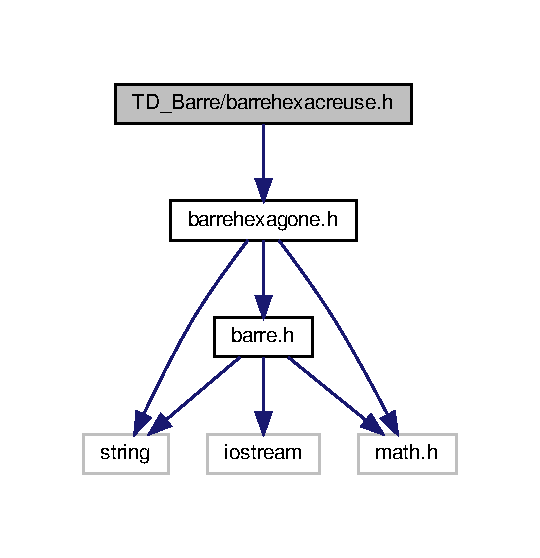
\includegraphics[width=259pt]{barrehexacreuse_8h__incl}
\end{center}
\end{figure}
Ce graphe montre quels fichiers incluent directement ou indirectement ce fichier \+:
\nopagebreak
\begin{figure}[H]
\begin{center}
\leavevmode
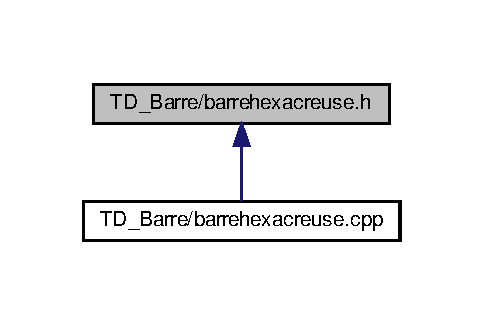
\includegraphics[width=232pt]{barrehexacreuse_8h__dep__incl}
\end{center}
\end{figure}
\subsection*{Classes}
\begin{DoxyCompactItemize}
\item 
class \hyperlink{classbarre_hexa_creuse}{barre\+Hexa\+Creuse}
\begin{DoxyCompactList}\small\item\em The \hyperlink{classbarre_hexa_creuse}{barre\+Hexa\+Creuse} class. \end{DoxyCompactList}\end{DoxyCompactItemize}

\hypertarget{barrehexagone_8cpp}{}\section{Référence du fichier T\+D\+\_\+\+Barre/barrehexagone.cpp}
\label{barrehexagone_8cpp}\index{T\+D\+\_\+\+Barre/barrehexagone.\+cpp@{T\+D\+\_\+\+Barre/barrehexagone.\+cpp}}
{\ttfamily \#include \char`\"{}barrehexagone.\+h\char`\"{}}\newline
Graphe des dépendances par inclusion de barrehexagone.\+cpp\+:
\nopagebreak
\begin{figure}[H]
\begin{center}
\leavevmode
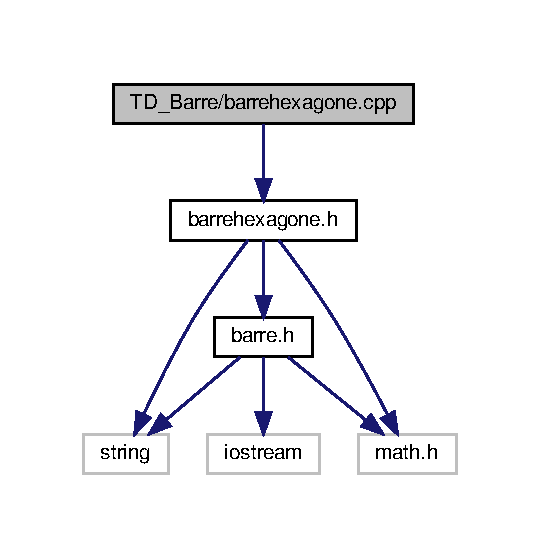
\includegraphics[width=259pt]{barrehexagone_8cpp__incl}
\end{center}
\end{figure}

\hypertarget{barrehexagone_8h}{}\section{Référence du fichier T\+D\+\_\+\+Barre/barrehexagone.h}
\label{barrehexagone_8h}\index{T\+D\+\_\+\+Barre/barrehexagone.\+h@{T\+D\+\_\+\+Barre/barrehexagone.\+h}}
{\ttfamily \#include $<$string$>$}\newline
{\ttfamily \#include \char`\"{}barre.\+h\char`\"{}}\newline
{\ttfamily \#include $<$math.\+h$>$}\newline
Graphe des dépendances par inclusion de barrehexagone.\+h\+:
\nopagebreak
\begin{figure}[H]
\begin{center}
\leavevmode
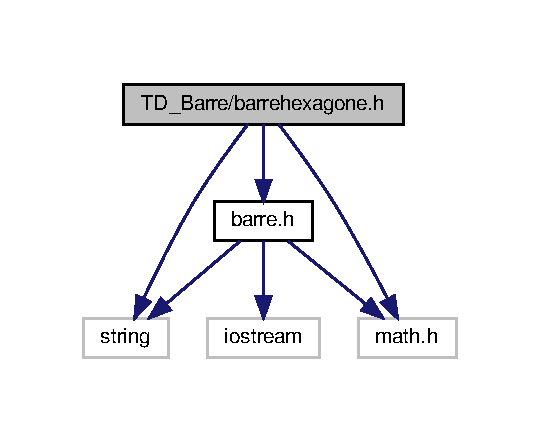
\includegraphics[width=259pt]{barrehexagone_8h__incl}
\end{center}
\end{figure}
Ce graphe montre quels fichiers incluent directement ou indirectement ce fichier \+:
\nopagebreak
\begin{figure}[H]
\begin{center}
\leavevmode
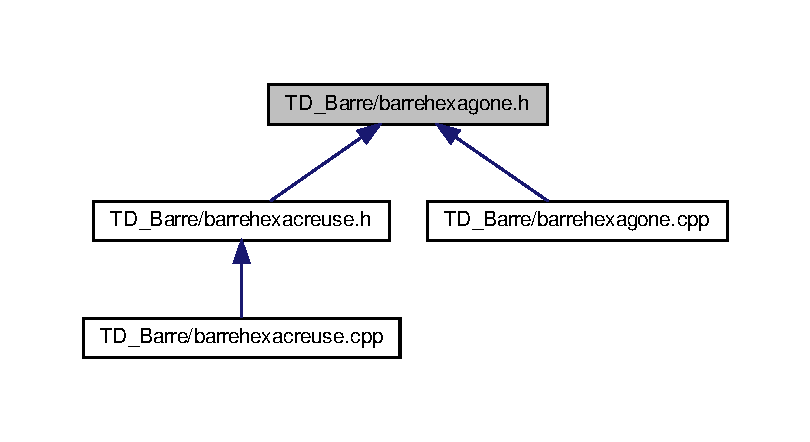
\includegraphics[width=350pt]{barrehexagone_8h__dep__incl}
\end{center}
\end{figure}
\subsection*{Classes}
\begin{DoxyCompactItemize}
\item 
class \hyperlink{classbarre_hexagone}{barre\+Hexagone}
\begin{DoxyCompactList}\small\item\em The \hyperlink{classbarre_hexagone}{barre\+Hexagone} class. \end{DoxyCompactList}\end{DoxyCompactItemize}

\hypertarget{barreoctogone_8cpp}{}\section{Référence du fichier T\+D\+\_\+\+Barre/barreoctogone.cpp}
\label{barreoctogone_8cpp}\index{T\+D\+\_\+\+Barre/barreoctogone.\+cpp@{T\+D\+\_\+\+Barre/barreoctogone.\+cpp}}
{\ttfamily \#include \char`\"{}barreoctogone.\+h\char`\"{}}\newline
Graphe des dépendances par inclusion de barreoctogone.\+cpp\+:
\nopagebreak
\begin{figure}[H]
\begin{center}
\leavevmode
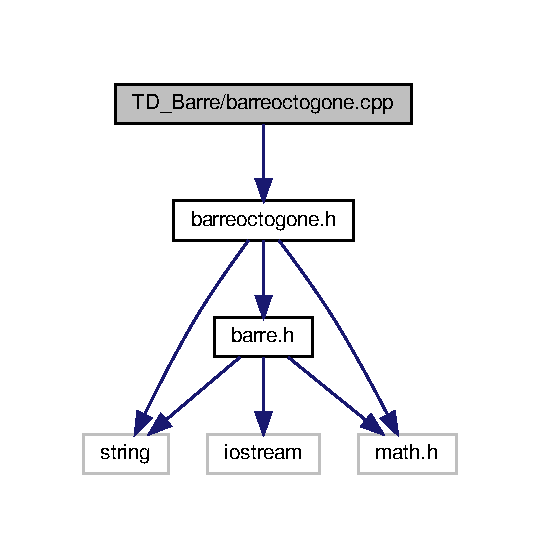
\includegraphics[width=259pt]{barreoctogone_8cpp__incl}
\end{center}
\end{figure}

\hypertarget{barreoctogone_8h}{}\section{Référence du fichier T\+D\+\_\+\+Barre/barreoctogone.h}
\label{barreoctogone_8h}\index{T\+D\+\_\+\+Barre/barreoctogone.\+h@{T\+D\+\_\+\+Barre/barreoctogone.\+h}}
{\ttfamily \#include $<$barre.\+h$>$}\newline
{\ttfamily \#include $<$math.\+h$>$}\newline
{\ttfamily \#include $<$string$>$}\newline
Graphe des dépendances par inclusion de barreoctogone.\+h\+:
\nopagebreak
\begin{figure}[H]
\begin{center}
\leavevmode
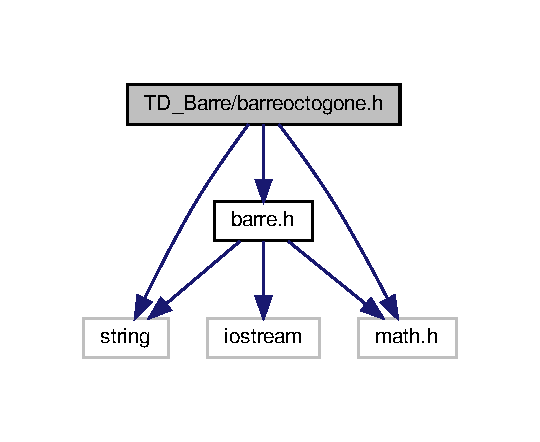
\includegraphics[width=259pt]{barreoctogone_8h__incl}
\end{center}
\end{figure}
Ce graphe montre quels fichiers incluent directement ou indirectement ce fichier \+:
\nopagebreak
\begin{figure}[H]
\begin{center}
\leavevmode
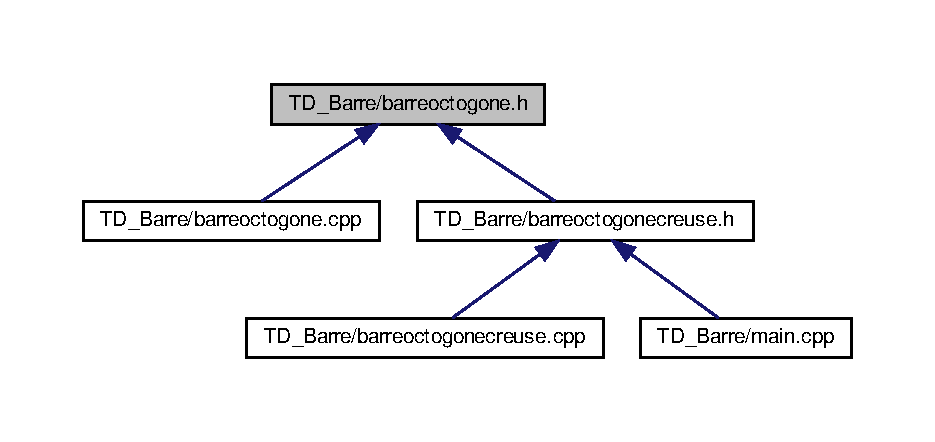
\includegraphics[width=350pt]{barreoctogone_8h__dep__incl}
\end{center}
\end{figure}
\subsection*{Classes}
\begin{DoxyCompactItemize}
\item 
class \hyperlink{classbarre_octogone}{barre\+Octogone}
\begin{DoxyCompactList}\small\item\em The \hyperlink{classbarre_octogone}{barre\+Octogone} class. \end{DoxyCompactList}\end{DoxyCompactItemize}

\hypertarget{barreoctogonecreuse_8cpp}{}\section{Référence du fichier T\+D\+\_\+\+Barre/barreoctogonecreuse.cpp}
\label{barreoctogonecreuse_8cpp}\index{T\+D\+\_\+\+Barre/barreoctogonecreuse.\+cpp@{T\+D\+\_\+\+Barre/barreoctogonecreuse.\+cpp}}
{\ttfamily \#include \char`\"{}barreoctogonecreuse.\+h\char`\"{}}\newline
Graphe des dépendances par inclusion de barreoctogonecreuse.\+cpp\+:
\nopagebreak
\begin{figure}[H]
\begin{center}
\leavevmode
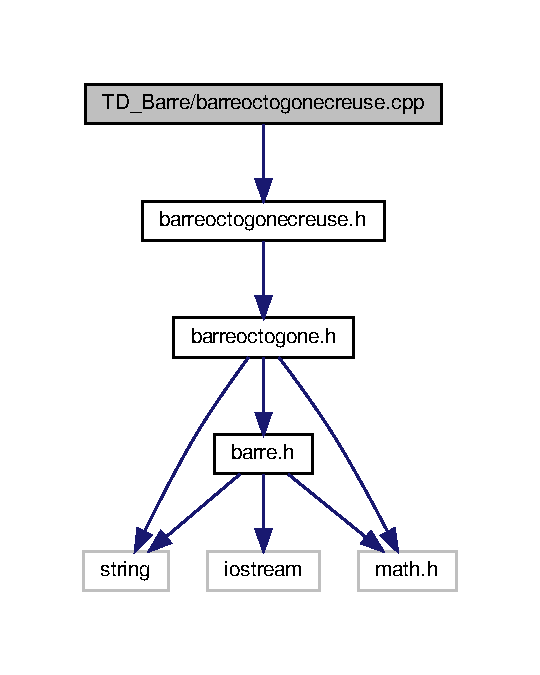
\includegraphics[width=259pt]{barreoctogonecreuse_8cpp__incl}
\end{center}
\end{figure}

\hypertarget{barreoctogonecreuse_8h}{}\section{Référence du fichier T\+D\+\_\+\+Barre/barreoctogonecreuse.h}
\label{barreoctogonecreuse_8h}\index{T\+D\+\_\+\+Barre/barreoctogonecreuse.\+h@{T\+D\+\_\+\+Barre/barreoctogonecreuse.\+h}}
{\ttfamily \#include \char`\"{}barreoctogone.\+h\char`\"{}}\newline
Graphe des dépendances par inclusion de barreoctogonecreuse.\+h\+:
\nopagebreak
\begin{figure}[H]
\begin{center}
\leavevmode
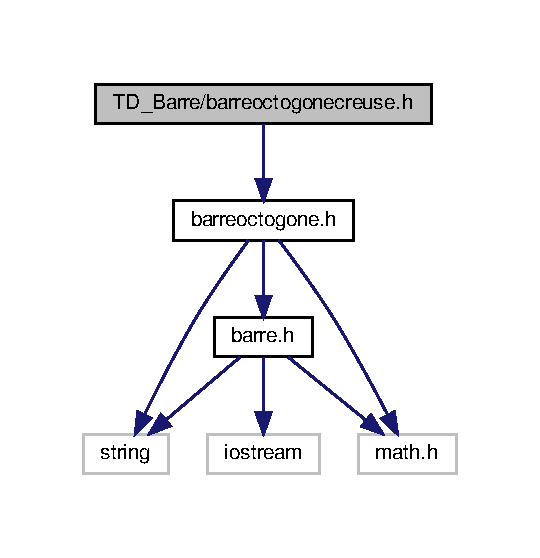
\includegraphics[width=259pt]{barreoctogonecreuse_8h__incl}
\end{center}
\end{figure}
Ce graphe montre quels fichiers incluent directement ou indirectement ce fichier \+:
\nopagebreak
\begin{figure}[H]
\begin{center}
\leavevmode
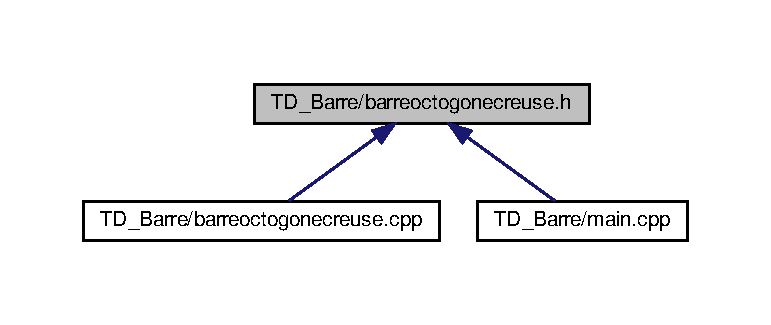
\includegraphics[width=350pt]{barreoctogonecreuse_8h__dep__incl}
\end{center}
\end{figure}
\subsection*{Classes}
\begin{DoxyCompactItemize}
\item 
class \hyperlink{classbarre_octogone_creuse}{barre\+Octogone\+Creuse}
\begin{DoxyCompactList}\small\item\em The \hyperlink{classbarre_octogone_creuse}{barre\+Octogone\+Creuse} class. \end{DoxyCompactList}\end{DoxyCompactItemize}

\hypertarget{barrerectangle_8cpp}{}\section{Référence du fichier T\+D\+\_\+\+Barre/barrerectangle.cpp}
\label{barrerectangle_8cpp}\index{T\+D\+\_\+\+Barre/barrerectangle.\+cpp@{T\+D\+\_\+\+Barre/barrerectangle.\+cpp}}
{\ttfamily \#include \char`\"{}barrerectangle.\+h\char`\"{}}\newline
Graphe des dépendances par inclusion de barrerectangle.\+cpp\+:
\nopagebreak
\begin{figure}[H]
\begin{center}
\leavevmode
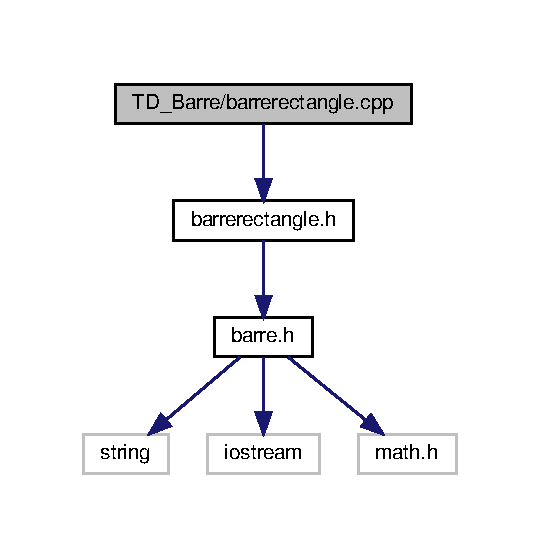
\includegraphics[width=259pt]{barrerectangle_8cpp__incl}
\end{center}
\end{figure}

\hypertarget{barrerectangle_8h}{}\section{Référence du fichier T\+D\+\_\+\+Barre/barrerectangle.h}
\label{barrerectangle_8h}\index{T\+D\+\_\+\+Barre/barrerectangle.\+h@{T\+D\+\_\+\+Barre/barrerectangle.\+h}}
{\ttfamily \#include \char`\"{}barre.\+h\char`\"{}}\newline
Graphe des dépendances par inclusion de barrerectangle.\+h\+:
\nopagebreak
\begin{figure}[H]
\begin{center}
\leavevmode
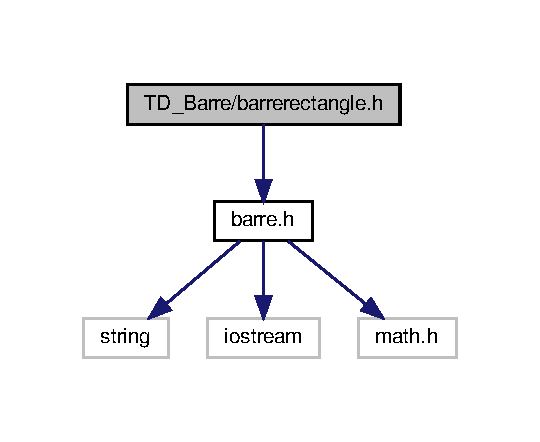
\includegraphics[width=259pt]{barrerectangle_8h__incl}
\end{center}
\end{figure}
Ce graphe montre quels fichiers incluent directement ou indirectement ce fichier \+:
\nopagebreak
\begin{figure}[H]
\begin{center}
\leavevmode
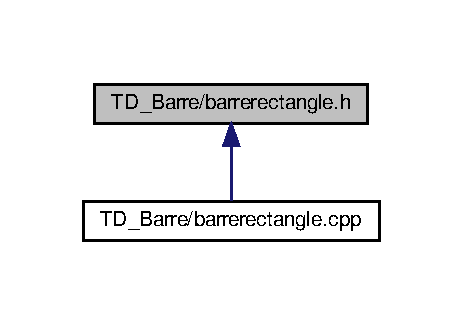
\includegraphics[width=222pt]{barrerectangle_8h__dep__incl}
\end{center}
\end{figure}
\subsection*{Classes}
\begin{DoxyCompactItemize}
\item 
class \hyperlink{classbarre_rectangle}{barre\+Rectangle}
\begin{DoxyCompactList}\small\item\em The \hyperlink{classbarre_rectangle}{barre\+Rectangle} class. \end{DoxyCompactList}\end{DoxyCompactItemize}

\hypertarget{barreronde_8cpp}{}\section{Référence du fichier T\+D\+\_\+\+Barre/barreronde.cpp}
\label{barreronde_8cpp}\index{T\+D\+\_\+\+Barre/barreronde.\+cpp@{T\+D\+\_\+\+Barre/barreronde.\+cpp}}
{\ttfamily \#include \char`\"{}barreronde.\+h\char`\"{}}\newline
Graphe des dépendances par inclusion de barreronde.\+cpp\+:
\nopagebreak
\begin{figure}[H]
\begin{center}
\leavevmode
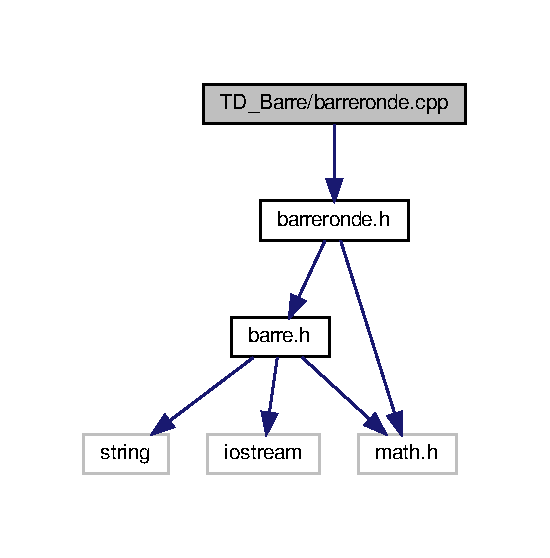
\includegraphics[width=264pt]{barreronde_8cpp__incl}
\end{center}
\end{figure}

\hypertarget{barreronde_8h}{}\section{Référence du fichier T\+D\+\_\+\+Barre/barreronde.h}
\label{barreronde_8h}\index{T\+D\+\_\+\+Barre/barreronde.\+h@{T\+D\+\_\+\+Barre/barreronde.\+h}}
{\ttfamily \#include \char`\"{}barre.\+h\char`\"{}}\newline
{\ttfamily \#include $<$math.\+h$>$}\newline
Graphe des dépendances par inclusion de barreronde.\+h\+:
\nopagebreak
\begin{figure}[H]
\begin{center}
\leavevmode
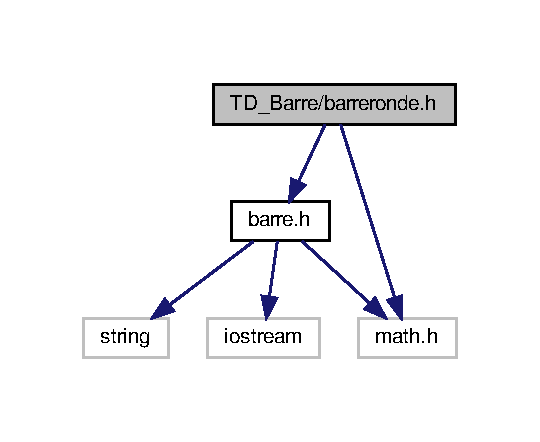
\includegraphics[width=259pt]{barreronde_8h__incl}
\end{center}
\end{figure}
Ce graphe montre quels fichiers incluent directement ou indirectement ce fichier \+:
\nopagebreak
\begin{figure}[H]
\begin{center}
\leavevmode
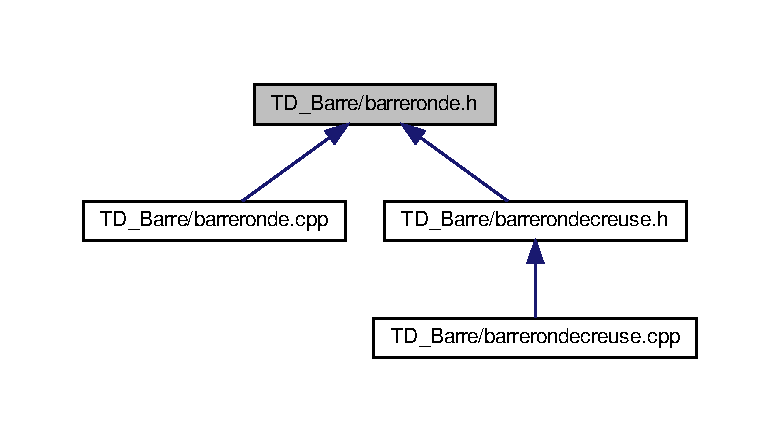
\includegraphics[width=350pt]{barreronde_8h__dep__incl}
\end{center}
\end{figure}
\subsection*{Classes}
\begin{DoxyCompactItemize}
\item 
class \hyperlink{classbarre_ronde}{barre\+Ronde}
\begin{DoxyCompactList}\small\item\em The \hyperlink{classbarre_ronde}{barre\+Ronde} class. \end{DoxyCompactList}\end{DoxyCompactItemize}

\hypertarget{barrerondecreuse_8cpp}{}\section{Référence du fichier T\+D\+\_\+\+Barre/barrerondecreuse.cpp}
\label{barrerondecreuse_8cpp}\index{T\+D\+\_\+\+Barre/barrerondecreuse.\+cpp@{T\+D\+\_\+\+Barre/barrerondecreuse.\+cpp}}
{\ttfamily \#include \char`\"{}barrerondecreuse.\+h\char`\"{}}\newline
Graphe des dépendances par inclusion de barrerondecreuse.\+cpp\+:
\nopagebreak
\begin{figure}[H]
\begin{center}
\leavevmode
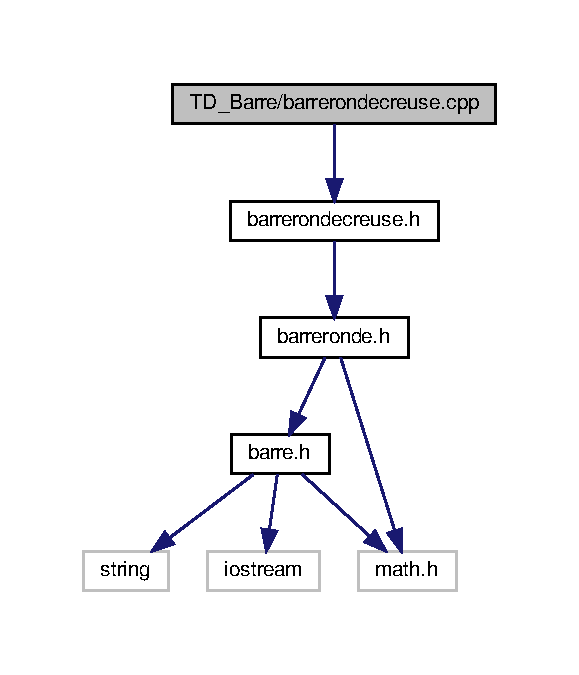
\includegraphics[width=278pt]{barrerondecreuse_8cpp__incl}
\end{center}
\end{figure}

\hypertarget{barrerondecreuse_8h}{}\section{Référence du fichier T\+D\+\_\+\+Barre/barrerondecreuse.h}
\label{barrerondecreuse_8h}\index{T\+D\+\_\+\+Barre/barrerondecreuse.\+h@{T\+D\+\_\+\+Barre/barrerondecreuse.\+h}}
{\ttfamily \#include \char`\"{}barreronde.\+h\char`\"{}}\newline
Graphe des dépendances par inclusion de barrerondecreuse.\+h\+:
\nopagebreak
\begin{figure}[H]
\begin{center}
\leavevmode
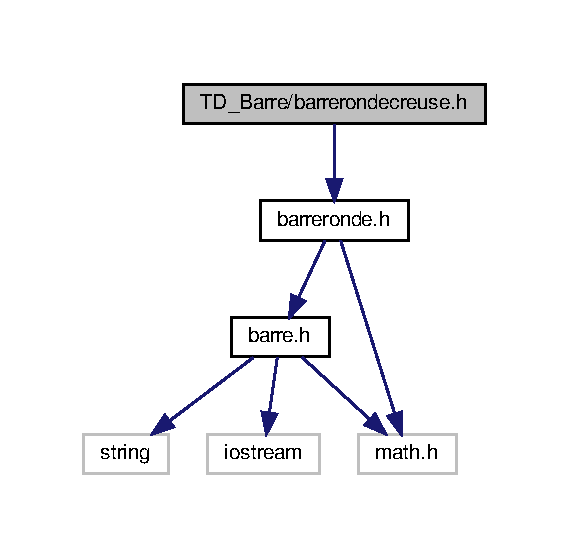
\includegraphics[width=273pt]{barrerondecreuse_8h__incl}
\end{center}
\end{figure}
Ce graphe montre quels fichiers incluent directement ou indirectement ce fichier \+:
\nopagebreak
\begin{figure}[H]
\begin{center}
\leavevmode
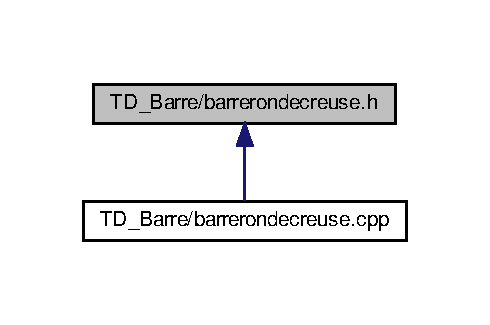
\includegraphics[width=235pt]{barrerondecreuse_8h__dep__incl}
\end{center}
\end{figure}
\subsection*{Classes}
\begin{DoxyCompactItemize}
\item 
class \hyperlink{classbarre_ronde_creuse}{barre\+Ronde\+Creuse}
\begin{DoxyCompactList}\small\item\em The \hyperlink{classbarre_ronde_creuse}{barre\+Ronde\+Creuse} class. \end{DoxyCompactList}\end{DoxyCompactItemize}

\hypertarget{main_8cpp}{}\section{Référence du fichier T\+D\+\_\+\+Barre/main.cpp}
\label{main_8cpp}\index{T\+D\+\_\+\+Barre/main.\+cpp@{T\+D\+\_\+\+Barre/main.\+cpp}}
{\ttfamily \#include $<$iostream$>$}\newline
{\ttfamily \#include \char`\"{}barreoctogonecreuse.\+h\char`\"{}}\newline
Graphe des dépendances par inclusion de main.\+cpp\+:
\nopagebreak
\begin{figure}[H]
\begin{center}
\leavevmode
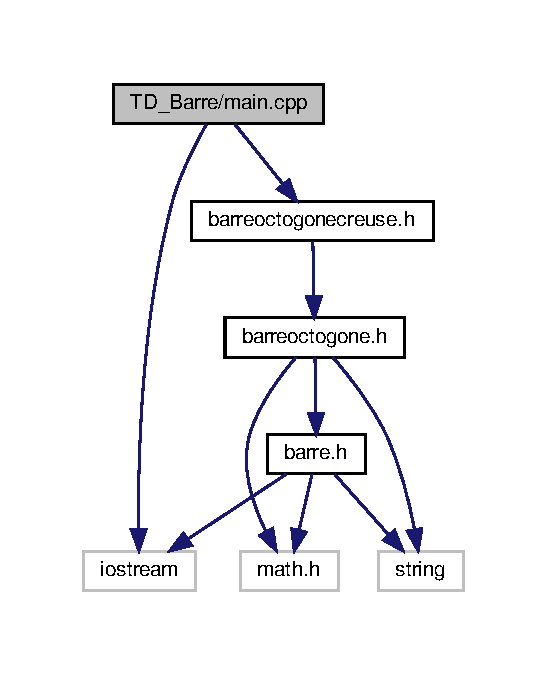
\includegraphics[width=263pt]{main_8cpp__incl}
\end{center}
\end{figure}
\subsection*{Fonctions}
\begin{DoxyCompactItemize}
\item 
int \hyperlink{main_8cpp_ae66f6b31b5ad750f1fe042a706a4e3d4}{main} ()
\begin{DoxyCompactList}\small\item\em main \end{DoxyCompactList}\end{DoxyCompactItemize}


\subsection{Documentation des fonctions}
\mbox{\Hypertarget{main_8cpp_ae66f6b31b5ad750f1fe042a706a4e3d4}\label{main_8cpp_ae66f6b31b5ad750f1fe042a706a4e3d4}} 
\index{main.\+cpp@{main.\+cpp}!main@{main}}
\index{main@{main}!main.\+cpp@{main.\+cpp}}
\subsubsection{\texorpdfstring{main()}{main()}}
{\footnotesize\ttfamily int main (\begin{DoxyParamCaption}{ }\end{DoxyParamCaption})}



main 

\begin{DoxyVersion}{Version}
1.\+0 
\end{DoxyVersion}
\begin{DoxyDate}{Date}
20/09/2019
\end{DoxyDate}
Programme Principal qui créer une barre en initialisant ses paramètres, Puis affiche sa Section et sa Masse \begin{DoxyReturn}{Renvoie}

\end{DoxyReturn}
Création d\textquotesingle{}un objet Barre\+Octogone\+Creuse

Affichage de la section de cette barre

Affichage de la Masse de cette Barre 
%--- End generated contents ---

% Index
\backmatter
\newpage
\phantomsection
\clearemptydoublepage
\addcontentsline{toc}{chapter}{Index}
\printindex

\end{document}
